% This is samplepaper.tex, a sample chapter demonstrating the
% LLNCS macro package for Springer Computer Science proceedings;
% Version 2.20 of 2017/10/04
%
\documentclass[runningheads]{llncs}
% 
\usepackage{array,xspace,multirow,hhline,graphicx,tikz,colortbl,tabularx,amsmath,amssymb,amsfonts}
\usepackage{thm-restate,thmtools}
\usepackage{xcolor}
\usepackage{booktabs}


\usepackage[sort,numbers]{natbib}
\usepackage{authblk}
% \renewcommand{\bibname}{References}
 \renewcommand{\bibsection}{\section*{References}}
 \makeatletter 
 \renewcommand\@biblabel[1]{#1} 
 \makeatother

\usepackage{xfrac}
\usepackage{caption}
\usepackage{subcaption}
\captionsetup{compatibility=false}
\usepackage{collcell} 

\usepackage{wrapfig} 
\usepackage{bbm}  
\usepackage{verbatim,ifthen} 
\usepackage{pifont} 

\usepackage{nicefrac}  
\usepackage[normalem]{ulem}
	\usepackage{varioref}

\usepackage{calc}
\newsavebox\CBox
\newcommand\hcancel[2][0.5pt]{%
  \ifmmode\sbox\CBox{$#2$}\else\sbox\CBox{#2}\fi%
  \makebox[0pt][l]{\usebox\CBox}%  
  \rule[0.5\ht\CBox-#1/2]{\wd\CBox}{#1}}

\tikzset{
  jumpdot/.style={mark=*,solid},
  excl/.append style={jumpdot,fill=white},
  incl/.append style={jumpdot,fill=black},
  rexcl/.append style={jumpdot,color=red,fill=white},
  rincl/.append style={jumpdot,fill=black,color=red},
} 

\usepackage[ruled,vlined,linesnumbered]{algorithm2e} % For algorithms
\renewcommand{\algorithmcfname}{ALGORITHM}
\SetAlFnt{\small}
\SetAlCapFnt{\small}
\SetAlCapNameFnt{\small}
\SetAlCapHSkip{0pt}
\IncMargin{-\parindent}
\DeclareMathOperator*{\argmax}{arg\,max}
\DeclareMathOperator*{\argmin}{arg\,min}
\newcommand{\USC}[1]{\ifstrempty{#1}{\textrm{\textup{USC}}}{#1\textrm{\textup{-USC{}}}}}
\newcommand{\ESC}[1]{\ifstrempty{#1}{\textrm{\textup{ESC}}}{#1\textrm{\textup{-ESC{}}}}}
\newcommand{\USW}[1]{\ifstrempty{#1}{\textrm{\textup{USW}}}{#1\textrm{\textup{-USW{}}}}}
\newcommand{\ESW}[1]{\ifstrempty{#1}{\textrm{\textup{ESW}}}{#1\textrm{\textup{-ESW{}}}}}
\newcommand{\PO}{\textup{PO}}
\newcommand{\EFone}{\textrm{\textup{EF1}}}
\newcommand{\MMS}{\textrm{\textup{MMS}}} 
\newcommand{\EFX}{\textrm{\textup{EFX}}\xspace}
\newcommand{\OPT}{\mathsf{OPT}}
\newcommand{\ALG}{\mathsf{ALG}}


\newcommand{\calA}{\mathcal{A}}
\renewcommand{\emptyset}{\varnothing} 

\newtheorem{observation}{Observation}{}

	\newcommand{\pref}{\succsim\xspace}
	\newcommand{\spref}{\ensuremath{\succ}} 
	
	\newcommand\blfootnote[1]{%
  \begingroup
  \renewcommand\thefootnote{}\footnote{#1}%
  \addtocounter{footnote}{-1}%
  \endgroup
} 
\usepackage{mathtools}
\DeclarePairedDelimiter\ceil{\lceil}{\rceil}
\DeclarePairedDelimiter\floor{\lfloor}{\rfloor} 

\newcommand{\todo}[1]{\textcolor{red}{[Todo: #1]}}

   %\usepackage[subtle]{savetrees}

\definecolor{gray(x11gray)}{rgb}{0.75, 0.75, 0.75}
\def\colorModel{rgb} %You can use rgb or hsb
 
	\usepackage{boxedminipage}
\usepackage{xspace}

%\newcommand{\haris}[1]{{\color{red}(\textbf{Haris says:} #1)}\xspace}

\newcommand{\shivika}[1]{{\color{violet!70!pink}{Shivika says: }{#1} }}

\newcommand{\mash}[1]{{\color{blue}{Mash says: }{#1} }}

\newcommand{\nooutput}{\ensuremath{\emptyset}}

	\renewcommand{\Pr}[1]{\ensuremath{\operatorname{\mathbf{Pr}}\left[#1\right]}}
	\newcommand{\Prbig}[1]{\ensuremath{\operatorname{\mathbf{Pr}}\big[#1\big]}}
	\newcommand{\PrBig}[1]{\ensuremath{\operatorname{\mathbf{Pr}}\Big[#1\Big]}}
	\newcommand{\Pro}[1]{\ensuremath{\operatorname{\mathbf{Pr}}\left[#1\right]}}

	\newcommand{\Var}[1]{\ensuremath{\operatorname{\mathbf{Var}}\left[#1\right]}}
	\newcommand{\target}{{L}\xspace}

	\newcommand{\Ex}[1]{\ensuremath{\operatorname{\mathbf{E}}\left[#1\right]}}
	
\newcommand{\haris}[1]{\textcolor{red}{Haris says: #1}}
\newcommand{\harisnew}[1]{\textcolor{red}{ #1}}
			\newcommand{\pbDef}[3]{%
			\smallskip
			\noindent
			\begin{center}
			\begin{boxedminipage}{0.98 \columnwidth}
			#1\\[5pt]
			\begin{tabular}{l p{0.75 \columnwidth}}
			Input: & #2\\
			Question: & #3
			\end{tabular}
			\end{boxedminipage}
			\end{center}
			\smallskip
			}

\newcommand{\midd}{\mathbin{:}}
	\newcommand{\ie}{i.e.,\xspace}
	\usepackage{xr}
		\newcommand{\M}{\mathcal{M}}
\usepackage[capitalise,noabbrev]{cleveref}
\newcommand{\G}{\mathcal{G}}
\newcommand{\E}{\mathcal{E}}
\usepackage{geometry}
\geometry{
  a4paper,         % or letterpaper
  textwidth=15cm,  % llncs has 12.2cm
  textheight=22cm, % llncs has 19.3cm
  heightrounded,   % integer number of lines
  hratio=1:1,      % horizontally centered
  vratio=2:3,      % not vertically centered
}
 
\Crefname{observation}{Observation}{Observations}   

\begin{document}
%

\title{Maximum Welfare Allocations under Quantile Valuations}

%\titlerunning{Allocations under Quantile Values }
% If the paper title is too long for the running head, you can set
% an abbreviated paper title here
%

\author{Haris Aziz, Shivika Narang, Mashbat Suzuki}

%\author{Haris Aziz
%}
%%
%\authorrunning{..}
%
%\institute{UNSW Sydney\\
%\email{haris.aziz@unsw.edu.au}}
%
%\author{Haris Aziz
%}
%%
%\authorrunning{..}
%
%\institute{UNSW Sydney\\
%\email{haris.aziz@unsw.edu.au}}
\institute{UNSW Sydney
\email{\{haris.aziz, s.narang, mashbat.suzuki\} @unsw.edu.au}}


\maketitle              % typeset the header of the contribution
%

		%File: formatting-instructions-latex-2023.tex
%release 2023.0


\begin{abstract}
We propose a new model for aggregating preferences over a set of indivisible items based on a quantile value. In this model, each agent is endowed with a specific quantile, and the value of a given bundle is defined by the corresponding quantile of the individual values of the items within it.
Our model captures the diverse ways in which agents may perceive a bundle, even when they agree on the values of individual items.  It enables richer behavioral modeling that cannot be easily captured by additive valuation functions.
We study the problem of maximizing utilitarian and egalitarian welfare within the quantile-based valuation setting. For each of the welfare functions, we analyze the complexity of the objectives. Interestingly, our results show that the complexity of both objectives varies significantly depending on whether the allocation is required to be balanced.  We provide near-optimal approximation algorithms for utilitarian welfare, and for egalitarian welfare, we present exact algorithms whenever possible. 
\end{abstract}

\section{Introduction} 

Consider a setting where submitted papers (items) need to be allocated among a set of reviewers (agents). Reviewers may have different levels of satisfaction with a given set of papers assigned to them, even when they agree on the quality of the papers. For instance, one reviewer’s perception of the allocation might depend on the most unpleasant task they need to undertake. Another reviewer, however, might not be concerned about the workload or the most unpleasant paper; their satisfaction could instead depend on the most interesting and inspiring paper in the set. 
%
Both opinions can be captured by different quantile values for the set of items (papers) assigned to the agents. The pessimistic reviewer bases their satisfaction on the lowest quantile, whereas the more optimistic reviewer bases their satisfaction on the highest quantile. Similarly, other types of reviewers may base their satisfaction on a different quantile value, such as the median paper in their batch. 
We introduce a novel valuation class, termed \textit{ quantile valuations}, which encompasses the aforementioned scenarios. In this framework, each agent is endowed with a specific quantile value  $\tau\in[0,1]$, and the value that she assigns for a bundle $S$ is the $\tau$-quantile of the distribution of item values in $S$. 
Returning to the conference paper assignment example, the pessimistic reviewer corresponds to an agent with quantile  $\tau=0$, whereas the optimistic reviewer corresponds to a quantile $\tau=1$. 


Quantiles are widely used across data analysis and statistics because they provide a robust description of value distributions. Compared to measures like average or total/gross, most quantile based measures are significantly less susceptible to outliers. As a result, quantiles are commonly used in practical settings, in measures like median household income, median age, and median house price in a given neighborhood etc.
%
Quantiles have also been used in decision theory to model agent preferences in settings where agents have preferences over stochastic outcomes. Specifically, quantiles have been considered in settings where an agent faces a choice of actions, each yielding a distribution over outcomes. Here, modeling the agent's choice as a quantile maximizer has been shown to provide a better approximation of human behavior than modeling them as an  expected utility maximizer \citep{DeGa2019dynamic,DeGa2022static}. 
%The class of valuations that we propose, \textit{ quantile valuations}, offers a quantile-based preference model in the context of indivisible item allocation.
Based on such quantile-based preferences, we introduce {\em quantile valuations} to the problem of allocating indivisible items.

Applications like assigning conference submissions to reviewers demand that agents receive similar sized sets. In contrast, when comparing the welfare of cities and neighborhoods, there is no guarantee that the underlying populations are of similar size. As a result, we give results for both the space of {\em balanced} allocations as well as for {\em all} allocations.
%
%Inspired by this, we explore a quantile-based preference model in the context of allocating indivisible items. While allocations of indivisible items are  well studied (see \cite{AAB+2022fair} for a survey), the typical assumption is that agents have additive or other monotone  valuations. 
%%
%Another departure from the standard allocation setting is the type of allocations considered. We shall often focus on {\em balanced allocations} where agents must receive the same number of items. 
%


%%%%%%%%%%%%%%%%%%%%%%%%%%%%%%%%%%%%%%%%%%%%%%%%%%%%%%%%%%%%%%%%
%%%%%%%%%%%%%%%%%%%%%%%%%%%%%%%%%%%%%%%%%%%%%%%%%%%%%%%%%%%%%%%% 

\subsection{Our Results}

\begin{table*}[t]
	\centering
    \crefname{theorem}{Thm.}{Thm.}
	\begin{tabular}{ccccc}
		\hline 
		&\textbf{ Objective}\quad    &            & \quad \quad \textbf{Our Results  }\quad  \quad  &        \\
		\hline         
        \multirow{3}{*}{\textbf{Balanced}}   &\multirow{2}{*}{\textbf{USW}} & Algorithms &  $\USW{\min(\frac{m}{n}+1,n)}^{\dagger}$  &  (\cref{thm:balUSWgreedy}) \\
		&                                     & Complexity      & \quad  NP-h to find $\USW{O\left(\frac{m/n}{\log (m/n)} \right)}$, when $m \leq n^2$  &(\cref{thm:hardnessUSW:Balanced})     \\
		&\textbf{ESW} &Algorithms & in  P$^{\dagger}$ & (\cref{thm:balESW})   \\ 
		\hline
		\multirow{4}{*}{\textbf{Unbalanced}} &\multirow{2}{*}{\textbf{USW}}& Algorithms      & $\USW{(1+\frac{1}{n-1})}^{\dagger}$ & (\cref{thm:scapegoat})  \\
		&                               & Complexity      & NP-h    & (\cref{thm:NP-USW} )   \\
		&\multirow{2}{*}{\textbf{ESW}} &Algorithms      & in  P when $\tau \in \{0,\sfrac{1}{3},\frac{t}{t+1},1\}$,  for any $t\in \mathbb{Z}_+$ & (\cref{thm:ESWunbal})\\
		&                               & Complexity      & \quad  NP-h   when  $\tau \in \{\sfrac{1}{t}\ |\ t\geq 4\}\cup (\sfrac{3}{8},\sfrac{2}{5}]\cup (\sfrac{5}{9},\sfrac{3}{5}]$  &(\cref{thm:ESWunbalNP})  \\
		\hline
		
	\end{tabular}
	\caption{Complexity of computing \USW{} and \ESW{} optimal allocation given $n$ agents and $m$ items. $\USW{\alpha}$ refers to an $\alpha$ approximation to the optimal \USW{}. Results marked with $\dagger$ hold when agents have heterogeneous quantiles. All other results require agents to have the same (homogeneous) quantile value of $\tau$.  }
	\label{tab:contributions}
\end{table*} 

We study the problem of maximizing welfare for agents with quantile valuations. %When it is clear from the context, we refer to this class simply as quantile valuations to avoid verbosity. 
Under quantile valuations, each agent $i$ specifies their value for individual items and a quantile value $\tau_i\in [0,1]$. Given a bundle $B$, agent $i$'s value for $B$ is the $\tau_i$th quantile of the values of the items in $B$. We provide comprehensive results on  {\em utilitarian social welfare }(\USW{}) (see for e.g. \citet{Hars1955cardinal}), which captures efficiency, and {\em egalitarian social welfare} (\ESW{}) (see for e.g. \citet{Moul2004fair}), which captures fairness. 
We study each objective both with and without the balancedness requirement.
%A balanced allocation is one in which each agent receives an equal number of items, i.e., each agent receives $m/n$ items, where  $m$ is the number of items and $n$ is the number of agents $n$.
Our results for goods are summarized in \cref{tab:contributions}. 
Many of our results for goods also extend to  chores; however, some do not. %These exceptions, along with additional results for chores, are explained later.



%\haris{Is the table referenced in the contributions?}

\paragraph{Utilitarian Welfare.}  
We first show that  the problem of maximizing the Utilitarian Social Welfare is NP-hard for both balanced and all allocations. Over balanced allocations (where each agent receives $m/n$ items), we prove that it is NP-hard to approximate the optimal \USW{}  within a factor $O(\frac{m/n}{\log (m/n)})$ for instances with $m\leq n^2$. We then present  a $\min(\frac{m}{n}+1,n)$-approximation algorithm, which matches the hardness of approximation bound asymptotically. 

In the setting without constraints on the allocation, we present a $\left( 1+\frac{1}{n-1}\right)$-approximation algorithm to the optimal $\USW{}$. Our results thus demonstrate that the complexity of both problems differs significantly depending on whether the allocations are required to be balanced.


\paragraph{Egalitarian Welfare.} 

In the setting where allocations are constrained to be balanced, we prove that \ESW{} optimal allocations can be computed in polynomial time, even when agents have arbitrary heterogeneous quantiles. This is in contrast to \USW{}, where we have hardness of approximation. 

When not restricted to balanced allocations, we show that the complexity of maximizing \ESW{} is highly dependent on the agents' quantile values. Specifically, we prove that when agents have homogeneous quantiles $\tau$, the problem is solvable in polynomial time for $\tau \in \{ 0, \sfrac{1}{3}, \sfrac{1}{2}, \sfrac{t}{t+1}, 1 \ | \  t \in \mathbb{Z}_+ \}$. In contrast,  for $\tau \in \{\sfrac{1}{t} \ |\ t \geq 4 \} \cup (\sfrac{3}{8}, \sfrac{2}{5}] \cup (\sfrac{5}{9}, \sfrac{3}{5}]$, the problem becomes NP-hard, and  no multiplicative approximation is possible. Our results demonstrate that, for \ESW{}, the tractable and intractable values of $\tau$ {\em interlace}. % with each other.

%
%These results were obtained by a general reduction which shows that, when considering  \ESW{} optimal allocations, it is suffices to restrict to valuations where each agent assigns binary values to each item, these results  may prove useful for further studies on quantile valuations. 

\paragraph{Identical Valuations.} When all agents have the same valuation function, the strong intractability results for maximum \USW{} under balanced allocations and maximum \ESW{} over all allocations can be overcome. Due to space constraints, we defer this discussion to \cref{sec:identical}.


\paragraph{Chores.}  For chores, under balanced allocations, the problem of minimizing {\em utilitarian social cost} (\USC{}) is NP-hard by using similar reductions as in the goods setting. Further, we show that without the balancedness constraint, the problem of  minimizing \USC{} is NP-hard to approximate to  factor better than $(1-o(1))\log m$. 
This establishes a clear separation between the goods and chores settings.%, as a $(1+\frac{1}{n-1})$-approximation was achievable in the goods setting. 


For the problem of finding a minimum {\em egalitarian social cost} (\ESC{}) balanced allocation, the algorithmic ideas developed for the goods setting extend to the chores setting, providing a polynomial-time algorithm for this problem. However, without the balancedness constraint, many of the algorithmic results for \ESW{} no longer apply. For instance, for goods, under a homogeneous quantile of $\tau=\sfrac{1}{2}$, maximum \ESW{} is solvable in polynomial time. However, the equivalent problem for chores is NP-hard. This once again highlights a difference between the goods and chores settings.

%%%%%%%%%%%%%%%%%%%%%%%%%%%%%%%%%%%%%%%%%%%%%%%%%%%%%%%%%%%%%%%%
%%%%%%%%%%%%%%%%%%%%%%%%%%%%%%%%%%%%%%%%%%%%%%%%%%%%%%%%%%%%%%%% 


\subsection{Related Work}
We defer an extended review of relevant work to \cref{app:relwork}. %Here, we  summarize the context for our paper.



 \paragraph{Quantile based preferences. } Quantile based preferences are well-established in mathematical economics and social choice theory. %\cite{DeGa2019dynamic,DeGa2022static} show that quantile preferences are a more accurate model of real-life behavior of agents in randomized settings over expected utility. 
 %
 Our proposed  valuations are a generalization of \textit{preference set extensions} that lift preferences over individual items to a set of items. The study of preference set extensions has a long-standing history in social choice theory~\citep{BBP04a} and has been applied to hedonic coalition formation games~\citep{CeHa2003computational,CeHa2004stable}, committee selection~\citep{AzMo20a} and multidimensional matchings \citep{HNR2025strategyproof}. %Typically, either the best or worst alternative in the proposed solution dictates the preferences.  %
 %Typical preference set extensions are either {\em best} or {\em worst} which correspond to quantile value $\tau=1$ and $\tau=0$ respectively in our model. 
 We discuss these in detail in \cref{app:relwork}, along with alternate generalizations of preference set extensions. %Among them, one is called the \textit{best set extension} in which the sets are compared based on the best item in each set. One is called the \textit{worst set extension},   in which the sets are compared based on the best item in each set. The best and worst extension correspond to the $\tau=1$ and $\tau=0$ in our model. 

 

\paragraph{Allocating Indivisible Items.} The problem of allocating indivisible items fairly and/or efficiently is very well studied (See \cite{AAB+2022fair} for a survey). Existing literature almost exclusively assumes that aggregated preferences are monotone, very often, additive\citep{CKM+2019unreasonable,ACIW2022fair}. Some also consider arbitrary (not necessarily monotone) valuations \citep{BBB+2024envy,BBPP2024nearly}. Our proposed valuations are non-monotone for most quantiles.  
%
Restricted cardinality allocations have been explored for additive valuations \citep{SHS2023efficient,BiBa2018fair,CaNa2024repeatedly}. %The valuations here are additive.   

%%%%%%%%%%%%%%%%%%%%%%%%%%%%%%%%%%%%%%%%%%%%%%%%%%%%%%%%%%%%%%%%
%%%%%%%%%%%%%%%%%%%%%%%%%%%%%%%%%%%%%%%%%%%%%%%%%%%%%%%%%%%%%%%%
%%%%%%%%%%%%%%%%%%%%%%%%%%%%%%%%%%%%%%%%%%%%%%%%%%%%%%%%%%%%%%%% 

\section{Model}

We shall use $[t]=\{1,\cdots, t\}$ for any $t\in \mathbb{Z}_+$.

We consider a setting with  a set of agents $N$ s.t. $|N|=n$ and a set of items $M$, s.t. $|M|=m$. Each agent  $i\in N$ has a valuation function $v_i$ over $M$.  Informally, a valuation function is $\tau$ quantile valuation, for $\tau\in[0,1]$, if the value assigned to  a bundle $S$ is determined by the $\tau$ quantile of the distribution of item values in $S$. We now provide a formal definition of this valuation class.  

\begin{definition}[Quantile Valuations]
    Given a set of indivisible items $M$, we say that $v_i:2^M\rightarrow \mathbb{R}$ is a $\tau$ quantile for $\tau_i\in [0,1]$, if for any subset $S\subseteq M$, we have that \[v_i(S)= \min_{g\in S} \Bigg\{v_i(g): \frac{|\{g'\in S:v_i(g')\leq v_i(g)\}|}{|S|}\geq \tau_i\Bigg\}  \]    
\end{definition}

An equivalent way of defining quantile valuations is to say that $v_i$ is a $\tau_i$ quantile for $\tau_i \in [0,1]$ if for any subset $S\subseteq M$ where $g_{i_{1}},\cdots,g_{i_{|S|}}$ are the items in $S$ s.t. $v_i(g_{i_1})\leq \cdots \leq v_i(g_{i_{|S|}})$ and $v_i(S)=v_i(g_{i_{\lceil \tau |S| \rceil} })$ if $\tau_i>0$, otherwise, $v_i(S)=v_i(g_{i_1})$. In particular, if $\tau_i$ is $0$, the agent values the given set as much as their least favorite item and if $\tau_i$ is $1$, they value it as much as their most favorite item.    

We shall use $\tau_i$ to denote the quantile of agent $i$. When all agents have the same quantile, we shall simply use $\tau$. Unless otherwise specified, assume that all agents have the same quantile $\tau\in [0,1]$.  Consequently, an instance of quantile allocations can be expressed by the tuple $I=\langle N, M, v, \tau \rangle$. %One benefit of this definition is that despite being non-monotone, the function does not require an oracle to specify the value on the subsets of items.  %, or 


Each item must be allocated to some agent. Formally, an allocation $A=(A_1,\cdots, A_n)$ is an $n$-partition of $M$, with $A_i$ being the set of items assigned to agent $i\in N$. We shall use $\Pi(n,M)$ to denote the set of all allocations that divide the items in $M$ among $n$ agents. Our aim is to allocations with maximum welfare.% We measure {efficiency} through {\em Utilitarian Social Welfare} and {fairness} through {\em Egalitarian Social Welfare}. 

\begin{definition}[Utilitarian Social Welfare (\USW{})]
Given an instance $I=\langle N,M, v, \tau \rangle$ and an allocation $A=(A_1,\cdots, A_n)$, the utilitarian social welfare is the sum of the values received by the agents.

\[\USW{}(A)=\sum_{i\in N}v_i(A_i)\]
\end{definition}

Given an instance $I=\langle N,M, v, \tau \rangle$, let $A^*$ be a maximum \USW{} allocation. We shall say that allocation $A$ is \USW{$\alpha$} for $\alpha \in [0,1]$, if $\USW{}(A)\geq  \alpha \USW{}(A^*)$. 

\begin{definition}[Egalitarian Social Welfare (\ESW{})]
Given an instance $I=\langle N,M,v, \tau \rangle$ and an allocation $A=(A_1,\cdots, A_n)$, the egalitarian social welfare is the minimum of the values incurred by the agents.

\[\ESW{}(A)=\min_{i\in N}v_i(A_i)\]    
\end{definition}

%In our model, the complexity of maximizing egalitarian welfare in general (with or without the balanced allocation restriction) is equivalent to maximizing \ESW{} when all $v_i(g)\in \{0,1\}$, that is with binary valuations. When valuations are binary, maximum \ESW{} is $1$, if and only if there is an allocation where all agents receive a value of $1$. Consequently, under binary valuations, any allocation that gives $\alpha>0$ approximation to the maximum \ESW{} would simply be a maximum \ESW{} allocation. As a result, we do not pursue any multiplicative approximations to \ESW{}. \shivika{Not sure if this paragraph should be here or can we skip stating this?}

\paragraph{Balanced Allocations}

Quantile valuations are very intuitive for settings where we insist on each agent getting an equal number of items, as in the case of assigning papers to reviewers in conferences. We shall consider both Utilitarian and Egalitarian Welfare with and without this requirement. 

When considering balanced allocations, we shall assume that the number of agents divides the number of items. That is, $m=kn$ for some $k\in \mathbb{Z}_+$. Thus, we shall look for allocations $A=(A_1,\cdots, A_n)$ where $|A_i|=k$. We shall use $\overline{\Pi}(n,M)$ to denote the set of all balanced allocations for instance $I$.

It is important to note that when we consider maximizing \USW{} or \ESW{} over balanced allocations, we are in fact finding a maximum welfare allocation from $\overline{\Pi}(I)$ alone. That is, we are not holding the allocations to the standard of maximum welfare under {\em any} allocation, balanced or otherwise. When not explicitly specified, assume any allocation in $\Pi(I)$.



\paragraph{Goods and Chores.} We shall say that an item $g\in M$ is a \textit{good}, if for all agents $v_i(g)\geq 0$. Analogously, we shall say that an item $g\in M$ is a \textit{chore}, if for all agents, $v_i(g)\leq 0$. 
%\haris{Please use backslash emph when introducing as term to be defined}
Unless specifically mentioned otherwise, the items we refer to will be goods.  When referring to chores, we shall often use the term disutilities with $d_i$ denoting agent $i$'s disutility where $d_i=-v_i$. Consequently, an instance of our problem can be denoted equivalently by $\langle N, M, d, \tau \rangle$ when considering an instance with chores.

When we consider instances with only chores, the social welfare notions become \textit{Utilitarian Social Cost (\USC{})} and \textit{Egalitarian Social Cost (\ESC{})}, respectively. Here, $\USC{}(A)= \sum_{i\in N} d_i(A_i)$ and $\ESC{}(A)=\max_{i\in N} d_i(A_i)$. We shall say that allocation $A$ is \USC{$\alpha$} for $\alpha \geq 1$, if $\USC{}(A)\leq  \alpha \USC{}(A^*)$ where $A^*$ has minimum \USC{}. %, where utilitarian social welfare is $\USW{}(A)=\sum_{i\in N}u_i(A_i)$ and egalitarian social welfare is $\ESC{}(A)=\max_{i\in N}u_i(A_i)$. The aim will be to maximize these welfare notions.

 



%%%%%%%%%%%%%%%%%%%%%%%%%%%%%%%%%%%%%%%%%%%%%%%%%%%%%%%%%%%%%%%%
%%%%%%%%%%%%%%%%%%%%%%%%%%%%%%%%%%%%%%%%%%%%%%%%%%%%%%%%%%%%%%%%
%%%%%%%%%%%%%%%%%%%%%%%%%%%%%%%%%%%%%%%%%%%%%%%%%%%%%%%%%%%%%%%% 

\section{Balanced Allocations} 

The requirement that the allocations be balanced is quite natural in practice, especially for the reviewer assignment context. Consequently, we first explore quantile valuations with the requirement that the allocations be balanced. Our results for \USW{} and \ESW{} lie in stark contrast with each other here. %We defer any omitted proofs to \cref{app:balanced}. 

%%%%%%%%%%%%%%%%%%%%%%%%%%%%%%%%%%%%%%%%%%%%%%%%%%%%%%%%%%%%%%%%
%%%%%%%%%%%%%%%%%%%%%%%%%%%%%%%%%%%%%%%%%%%%%%%%%%%%%%%%%%%%%%%%
 

 
\subsection{Utilitarian Social Welfare}\label{subsec:balUSW}
 We first show, when allocations are balanced,  that maximizing \USW{}  is NP-hard to approximate better than a factor of $O(\frac{m/n}{\log (m/n)})$. We then proceed to give a polynomial-time algorithm that matches hardness of approximation bound asymptotically. 

%%%%%%%%%%%%%%%%%%%%%%%%%%%%%%%%%%%%%%%%%%%%%%%%%%%%%%%%%%%%%%%%

 
\subsubsection{Hardness of Approximation}
In order to show hardness of approximation, we give a reduction from the $k$-\textup{\textsc{DimensionalMatching}}(kDM) problem. The kDM problem requires finding a maximum collection of disjoint edges in a k-partite hypergraph where each hyperedge has size $k$. The aim is to find a matching of maximum size. \citet{HSS03} showed that this problem is NP-hard to approximate to a factor better than $O(\frac{k}{\log k})$.

\begin{theorem}\label{thm:hardnessUSW:Balanced} 
 Given  instance $I=\langle N,M,v,\tau\rangle$ where $m< n^2$ and $m=kn$, it is NP-hard to find an $\USW{O\left(\frac{m/n}{\log (m/n)}\right)}$ balanced allocation.%there is no -factor approximation algorithm for maximizing \USW{} under a balancedness constraint, assuming P $\neq$ NP.
	\end{theorem}
\begin{proof}
	Given an instance of kDM, $\langle G=(X,H), \ell \rangle$, we create an instance of our problem %with $n$ agents and $m=kn$ items 
    as follows: For each edge $H_i\in H$, we create agent $i$. For each vertex $x\in X$, we create item $g_x$.  We can assume, without loss of generality, that each vertex is contained in at least one hyper-edge. Thus, we have that $|X|\leq k |H|$. To balance the item count, we introduce $k|H| - |X|$ dummy items $g'_1,\cdots, g'_{kn - |X|}$. 
    Thus, we have $n=|H|$ agents and the number of items is $m=k|H|$. As a result, we have that $m = kn$. Recall that balanced allocations require $k=\frac{m}{n}$ items to be allocated to each agent. 
    
    For each agent $i\in N$, we set $\tau_i=0$ for all $i\in N$. Now for $i$ and each $g_x$, if $x\in H_i$, we set $v_i(g_x)=1$ else, we set $v_i(g_x)=0$. Finally, for each $t\in [k|H| - |X|]$, set $v_i(g'_t)=0$.
     
	
	We now show that a matching of size $\ell$ in the kDM problem can be transformed into a balanced allocation whose \USW{} is at least $\ell$ in the reduced instance of our problem, and vice versa. Consider a matching $\mu$ of size $\ell$ in kDM. For each $H_i\in \mu$, allocate the items vertices in $H_i$. That is, $A_i=\{g_x|x\in H_i\}$. Arbitrarily allocate the remaining items, ensuring $|A_i|=k$. It is easy to see that $\USW{}(A)\geq \ell$. 
	
    Now consider a balanced allocation $A$ in the reduced instance with a \USW{} of $\ell$. As the maximum value for any agent is $1$, this implies that $\ell$ agents receive a value of $1$ from $A$. By construction, $v_i(A_i)=1$ only if $A_i$ contains {\em all} the items corresponding to the vertices in $H_i$. From here, it is easy to see that $\mu=\{H_i|v_i(A_i)=1\}$ is a matching of size $\ell$. 
    
    %We claim that these $\ell$ agents correspond to a matching of size $\ell$ in the kDM problem. To see this, recall that each agent receives a bundle of size $k$, and the only way for an agent to achieve a value of one is by receiving all items associated with their corresponding hyperedge. Since each item is allocated to exactly one agent, the hyperedges corresponding to the agents who receive a value of $1$ must be disjoint, and there are $\ell$ of them.
	
	\citet{HSS03} proved that there exists a class of instances with $k < n$ such that kDM is NP-hard to approximate within a factor of $O({k}/{\log(k)})$. Thus, we have hardness of approximation for instances where $m< n^2$. 
	\end{proof}
    
\begin{algorithm}[t]
	\KwIn{Instance with goods and heterogeneous quantiles $\langle N,M, v, \tau \rangle$  where $m=kn$}
	\KwOut{An allocation $A$}
	Initialize set of unallocated goods $P\gets M$\;
    Initialize set of unassigned agents $N'\gets N$\;
    Let $k_i\gets \min(k,k-\lceil \tau_i k\rceil+1) $\;
	\While{$P\neq \emptyset$}{
        For each $i\in N'$, let $S_i\gets \max\limits_{S : S\subseteq P , |S| = k_i  } v_i(S) $\;
		Let $i^*= \argmax\limits_{i\in N'} v_i(S_i)$\;
		$A_{i^*}\gets S_{i^*} $\;
		$P\gets P\setminus A_{i^*}$\;
		$N'\gets N' \setminus \{i^*\}$ \;
	}
    Allocate items in $P$ arbitrarily  s.t. $|A_i|=k$ for all $i\in N$\;
	\textbf{Return} $A$
	\caption{Greedy Algorithm for $\USW{\min(\frac{m}{n}+1,n)}$ }\label{alg:goods-USWbalanced}
\end{algorithm}

\subsubsection{Near-Optimal Algorithm}
We now provide an approximation algorithm that almost matches the lower bound placed by \cref{thm:hardnessUSW:Balanced}. The greedy algorithm (\cref{alg:goods-USWbalanced}) proceeds by iteratively allowing unassigned agents to ``demand" their best possible set from the unassigned items. We then choose the agent whose value for their demanded set is highest. We repeat this  until all items are assigned. 

\begin{restatable}{theorem}{USWgreedy}\label{thm:balUSWgreedy}
Given an instance $I=\langle N,M,v,\tau \rangle$ with $m=kn$ and heterogeneous quantiles, \cref{alg:goods-USWbalanced} returns a balanced allocation which is $\USW{\min(\frac{m}{n}+1,n)}$.
    
\end{restatable}

    
\begin{proof}
%Let the bundle size be $k=m/n$. ,  we show that \Cref{alg:goods-USWbalanced} has an approximation guarantee of $\min(k+1,n)$.   
Given $I$, let $A^*=(A^*_1,...,A^*_n)$ be a maximum \USW{} balanced allocation. Without loss of generality, we may assume that  $v_1(A^*_1) \geq v_2(A^*_2) \geq \dots \geq v_n(A^*_n)$. Let $i_t$ denote the agent who is allocated a bundle in the $t$-th iteration of the while loop, and let $A_{i_t}$ denote the corresponding bundle allocated to her under \cref{alg:goods-USWbalanced}. 

Let $k_i=\min(k,k-\lceil\tau_i k\rceil +1)$. That is, $k_i$ is minimum number of items in any $k$ sized bundle $B$ s.t. $v_i(g)\geq v_i(B)$. Recall that under the greedy algorithm, an agent ``demands" $k_i$ items. Let $k'=\max_i k_i$. Observe that $1\leq k'\leq k$.   We shall now show that the first $\lceil \frac{n}{k'+1}\rceil$ agents to receive a bundle will have value comparable to the value under specific bundles under $A^*$. \\

\noindent\textbf{Claim:} For each $t=1,\cdots, \lceil \frac{n}{k'+1} \rceil$, we have that the value of agent $i_t$, $v_{i_t}(A_{i_t}) \geq v_{(t-1)(k'+1)+1}(A^*_{(t-1)(k'+1)+1}) $.\\

\noindent{\em Proof of Claim.} %Assume, for contradiction, that there exists $\bar{t} \in [ \lceil \frac{n}{k+1} \rceil ]$ such that $v_{i_{\bar{t}}}(A_{i_{\bar{t}}}) < v_{(\bar{t}-1)(k+1)+1}(A^*_{(\bar{t}-1)(k+1)+1})$. Consider the smallest such $\bar{t}$. 
We shall prove this by induction. For $i_1$, as none of the items have been allocated, the best possible bundle $A_{i_1}$ must be such that $v_{i_1}(A_{i_1})\geq v_1(A_1^*)$. 

Suppose we have that for all $t\leq \bar{t}-1$, the claim holds. 
Let $L=\bigcup_{\ell\in [\bar{t}-1]} A_{i_\ell}$ be the set of items that are allocated up to the $(\bar{t}-1)$th iteration of the while loop. As at most $k'$ items are allocated in each iteration, we have that $|L|=k'(\bar{t}-1)$. It follows that in the worst case, the number of bundles under $A^*$ for which some item has already be allocated in $L$ is   $| \{ j\in [(\bar{t}-1)(k'+1)+1]  \ : \   A^*_j \cap L \neq  \emptyset \} | \leq |L| = k'(\bar{t}-1) $.

Consequently, we get that among the top $(\bar{t}-1)(k'+1)+1$ bundles under $A^*$, at least $\bar{t}$ bundles do not intersect with $L$.  Thus far, $\bar{t}-1$ bundles have been allocated. Consequently, at least one bundle and agent pair among these $\bar{t}$ unallocated bundles must remain available for selection .
Hence, we must have that $v_{i_{\bar{t}}}(A_{i_{\bar{t}}}) \geq v_{(t-1)(k'+1)+1}(A^*_{(t-1)(k'+1)+1})$.
%Since at the start of  the $\bar{t}$'th iteration, $\bar{t}-1$ agents haven been allocated a bundle, and there are at least $\bar{t}$ bundles from  $ \{A^*_r\}_{r\in [(\bar{t}-1)(k+1)+1]}$ that do not intersect $L$, by the pigeonhole principal, one of the agent-bundle pairs  in $ \{A^*_r\}_{r\in [(\bar{t}-1)(k+1)+1]}$ is available to be picked in the $\bar{t}$'th iteration. Thus, we have   However, this contradicts the initial assumption $v_{i_{\bar{t}}}(B_{i_{\bar{t}}}) < v_{(\bar{t}-1)(k+1)+1}(A^*_{(\bar{t}-1)(k+1)+1}) $. 
\qed %\\



\noindent  We can now prove the approximation guarantee. Let $\alpha=\min(k'+1,n)$. Observe that $\lceil \frac{n}{k'+1}\rceil=\lceil\frac{n}{\alpha}\rceil$. The \USW{} of $A$ is lower bounded by $\sum_{t=1}^{\lceil \frac{n}{k'+1} \rceil}  v_{i_t}(A_{i_t})$. From the proof of the claim, we know that 
%
\[\sum_{t=1}^{\lceil \frac{n}{\alpha} \rceil}  v_{i_t}(A_{i_t})\leq \sum_{t=1}^{\lceil \frac{n}{\alpha} \rceil}  v_{(t-1)(k'+1)+1}(A_{(t-1)(k'+1)+1}^*) \]
%
Recall that agents are ordered according to $A^*$, that is, $v_1(A^*_1)\geq \cdots\geq v_n(A^*)$. As a result, we get that $\USW{}(A^*)=\sum_{t\in [n]} v_t(A^*_t)\leq \alpha \sum_{t\in \lceil [\frac{n}{k'+1}] \rceil} v_{(t-1)(k'+1)+1}(A_{(t-1)(k'+1)+1}^*)$. From the claim, we know that this is less than or equal to $\alpha$ times the value obtained by the first $\lceil\frac{n}{k'+1}\rceil$ agents under \cref{alg:goods-USWbalanced}. Hence, $\USW{}(A)\geq \frac{\USW{}(A^*)}{\alpha}$.

Observe that when each agent demands $k_i<n-1$ items, we are guaranteed $\USW{(k'+1)}$ which may be even better than $\USW{(k+1)}$. However, when $k'\geq n-1$, the greedy algorithm can only guarantee $\USW{n}$. Consequently, for an arbitrary $I$, \cref{alg:goods-USWbalanced} is $\USW{\min (\frac{m}{n}+1,n)}$.
    \end{proof}





%%%%%%%%%%%%%%%%%%%%%%%%%%%%%%%%%%%%%%%%%%%%%%%%%%%%%%%%%%%%%%%%%%%%%
%%%%%%%%%%%%%%%%%%%%%%%%%%%%%%%%%%%%%%%%%%%%%%%%%%%%%%%%%%%%%%%%%%%%%

\subsection{Egalitarian Social Welfare}
We now move to maximizing egalitarian welfare. We begin with a very useful reduction, which facilitates all our algorithms for \ESW{}. We first show that whenever there is an algorithm to find an allocation with maximum Egalitarian Welfare under binary valuations, we can use it to find a maximum \ESW{} allocation under general non-negative valuations. %This proves useful in all our algorithmic results on \ESW{}. 
\begin{algorithm}[t]
  \KwIn{Instance with binary values and heterogeneous quantiles $\langle N,M, v, \tau \rangle$ s.t. $m=kn$ }
  \KwOut{Balanced Allocation $A$}
  Let $k_i=\min (k,k-\lceil \tau_i k\rceil -1)$\;
  Create bipartite graph $G=(X,Y,E)$ where $X$ contains $x_g$ for each $g\in M$,  
  $Y$ contains $y^i_1,\cdots y^i_{k_i}$ for each $i\in N$ and \\
  $(x_g,y^i_t)\in E$ only if $v_i(g)=1$, for each $i\in N,\, g\in M, t\in [k_i]$\;
  Let $\mu$ be a maximum cardinality matching in $G$\;
  \eIf{$|\mu|=|Y|$}{
        Initialize $A=(A_1,\cdots A_n)$ where $A_i\gets \{g|(x_g,y^i_t)\in \mu $ for some $ t\in [k_i]\}$ for each $i\in N$\;
        Allocate remaining items arbitrarily but ensuring $|A_i|=k$ for all $i\in N$\;
  }{
    Let $A$ be an arbitrary balanced allocation\;
  }
  \textbf{Return} $A$\;
   \caption{Max balanced \ESW{} for binary goods.}\label{alg:balESW}
\end{algorithm}

\begin{restatable}{lemma}{binreduction}\label{lem:binRednESW}
The problem of finding an allocation with \ESW{} at least $\nu\geq0$ over allocations in $\Pi'\subseteq \Pi(n,M)$ under heterogeneous quantiles reduces to maximizing \ESW{} over $\Pi'$ under binary  goods with heterogeneous quantiles. 
\end{restatable}

\begin{proof}
    Consider an arbitrary instance $I=\langle N,M,v,\tau \rangle$ and $\Pi'\subseteq \Pi(n,M)$ and a threshold $\nu$, s.t. we wish to find an allocation in $A\in \Pi'$ s.t. $\ESW{}(A)\geq \nu$. We can construct an alternate instance $I'=\langle N,M,v',\tau \rangle$ with binary valuations as follows: $v'_i(g)=1$ if and only if $v_i(g)\geq \nu$. We can now show that an allocation $A\in \Pi'$ has $\ESW{}(A)\geq \nu$ under $v$ if and only if $\ESW{}(A)=1$ under $v'$.

    Suppose we have an allocation $A\in \Pi'$ s.t. $A$ has $\ESW{}(A)\geq \nu$ under $v$. Thus, for each $i\in N$, $A_i$ must contain enough goods each with value at least $\nu$ so that $v_i(A_i)\geq \nu$. Thus, for the same quantile $\tau_i$, it must be that $v_i'(A_i)\geq 1$. Consequently, $\ESW{}(A)\geq 1$ under $v'$.

    Similarly, suppose we have an allocation $A\in \Pi'$ s.t. $A$ has $\ESW{}(A)\geq 1$ under $v'$. We can analogously see that $v_i'(A_i)\geq 1$ if and only if $v_i(A_i)\geq \nu$. As a result, it must be that $v_i(A_i)\geq \nu$ for each $i\in N$, and thus, $\ESW{}(A)\geq \nu$ under $v$.
\end{proof}

Given an algorithm $\textsc{ALG}$ which finds a maximum \ESW{} allocation over $\Pi'$ for binary goods. We can make a call to $\textsc{ALG}$ for a given value of $v_i(g)$ to see if an allocation with $\ESW{}$ at least $v_i(g)$ exists. Consequently, we can make at most $mn$ calls to $\textsc{ALG}$ to find a maximum $\ESW{}$ allocation over $\Pi'$ for the original instance.


This enables us to maximize \ESW{} over balanced allocations, even if the quantile values are heterogeneous. %Recall that under the balanced allocations requirement, %we assume that the number of items $m$ is a multiple of the number of agents. That is, $m=kn$. Consequently, under a balanced allocation, each agent must receive exactly $k=m/n$ items.
%We know from \cref{lem:binRednESW} that it is sufficient to consider a setting where agent values are binary. That is, 
We only consider a setting where $v_i(g) \in \{0,1\}$ for all $i\in N$ and all $g\in M$. Here, we shall try to see if an allocation with \ESW{} $1$ can exist. That is, all agents must get a value of $1$. In order to achieve this, we first make the following observation:

\begin{observation}\label{obs:basicBinVal}
    For an agent $i$ with quantile $\tau_i$ and binary valuations, a bundle $B\subseteq M$ where the size of $|B|=k$, the value for $B$, $v_i(B)=1$ if and only if there are at most $\lceil \tau_i k\rceil -1$ items in $B$ for which $i$ has value $0$. 
\end{observation}

This follows from the definition of quantile valuations. Thus, to have \ESW{} of $1$, each  $i\in N$ must receive at least $k_i=\min (k,k-\lceil \tau_i k\rceil +1)$ items of value $1$. Note that the min argument only comes in when $\tau_i=0$. 

We can check if this is possible using a simple maximum cardinality bipartite matching algorithm. This is shown in \cref{alg:balESW}. Here, we create a bipartite graph where for each $i\in N$, we create $k_i$ vertices, and for each $g\in M$ we create one vertex. We add an edge between $i$ and $g$ if $v_i(g)=1$. A matching of size $\sum_{i\in N}k_i$ exists if and only if the given instance has an allocation with \ESW{} of 1.


\begin{restatable}{proposition}{ESWbalanced}\label{prop:balancedESW}
Given $I=\langle N,M,v,\tau\rangle$ where $m=kn$ with binary goods and heterogeneous quantiles, \cref{alg:balESW} finds a maximum \ESW{} balanced allocation in polynomial time.  
\end{restatable}


\begin{proof}
   For an instance with binary goods, the maximum \ESW{} possible is $1$. %That is, the \ESW{} is maximized when all agents receive value $1$ from an allocation. 
%
    For a balanced allocation to have \ESW{} of $1$, from \cref{obs:basicBinVal} each $i\in N$ must receive at least $k_i=\min (k,k-\lceil \tau_i k\rceil +1)$ items which give $i$ value $1$. \cref{alg:balESW} checks if this is simultaneously possible for all $i\in N$. Let $A$ be the allocation returned by \cref{alg:balESW} on $I$. We shall now show that $\ESW{}(A)=1$ whenever a balanced allocation with \ESW{} $1$ exists for $I$. 

    Suppose a matching of size $\sum_{i\in N}k_i$ exists in the graph $G$  constructed in \cref{alg:balESW}. Consequently, $A_i$ contains at least $k_i$ items for which $i$ has value $1$. Thus, $\ESW{}(A)=1$.

    Conversely, let an allocation $A'$ with $\ESW{}(A')=1$ exist for the given instance. Then for each $i\in N$, $A'_i$ must contain at last $k_i$ items of value $1$ for $i$. Let $g_i^1\cdots g_i^{k_i}\in A_i'$ be distinct items s.t. $v_i(g_i^t)=1$ for all $t\in [k_i]$. Consider $\mu'=\{(x_{g_i^t},y^i_t)|t\in [k_i]\}$. Clearly, $|\mu'|=\sum_i k_i$. That is, a maximum cardinality matching of the required size must exist. As a result, the allocation returned by $A$ is s.t. $\ESW{}(A)=1$.

    \paragraph{Running Time.} The bipartite graph has $\sum_i k_i\leq kn=m$ vertices in $X$ and $m$ vertices in $Y$ and  thus, at most $m^2$ edges. A maximum cardinality matching on a bipartite graph can be found in polynomial time using the Ford-Fulkerson Algorithm. As a result, \cref{alg:balESW} runs in polynomial time.  
\end{proof}

As a consequence of \cref{lem:binRednESW} and \cref{prop:balancedESW}, we get the following theorem. 
\begin{theorem}\label{thm:balESW}
    Given $I=\langle N,M,v,\tau\rangle$ with heterogeneous quantiles  where $m=kn$, a balanced allocation with maximum \ESW{} can be found in polynomial time. 
\end{theorem}
%\shivika{Should this be a corollary or a theorem?}

%%%%%%%%%%%%%%%%%%%%%%%%%%%%%%%%%%%%%%%%%%%%%%%%%%%%%%%%%%%%%%%%
%%%%%%%%%%%%%%%%%%%%%%%%%%%%%%%%%%%%%%%%%%%%%%%%%%%%%%%%%%%%%%%%
%%%%%%%%%%%%%%%%%%%%%%%%%%%%%%%%%%%%%%%%%%%%%%%%%%%%%%%%%%%%%%%% 


\section{Unbalanced Allocations}

As previously mentioned, typical work on allocating indivisible items does not require allocations to be balanced. Thus, for completeness, we again explore welfare maximization, now over {\em all} allocations, beginning with utilitarian welfare. We find that while it possible to give significantly better guarantees on \USW{}, maximum \ESW{} now becomes intractable for a large subset of the quantiles. Any omitted proof are deferred to \cref{app:unbalanced}.


%%%%%%%%%%%%%%%%%%%%%%%%%%%%%%%%%%%%%%%%%%%%%%%%%%%%%%%%%%%%%%%%
%%%%%%%%%%%%%%%%%%%%%%%%%%%%%%%%%%%%%%%%%%%%%%%%%%%%%%%%%%%%%%%%

\subsection{Utilitarian Social Welfare}

We find that while maximizing \USW{} still remains intractable, we are able to circumvent hardness of approximation and achieve a near exact approximation algorithm that even works for heterogeneous quantiles. 

%%%%%%%%%%%%%%%%%%%%%%%%%%%%%%%%%%%%%%%%%%%%%%%%%%%%%%%%%%%%%%%%

\subsubsection{Intractability}

We first show that for non-identical agents with quantile $\tau=0$ for all agents, the problem of maximizing social welfare proves to be NP-hard for goods.  We give reduction from the \textup{\textsc{Exact3Cover}} problem, which is known to be NP-hard \citep{garey1979computers}.
\begin{restatable}{theorem}{USWreductionNP}\label{thm:NP-USW}
    Given instance $I=\langle N, M, v,\tau \rangle$ with goods finding a maximum \USW{} allocation is NP-complete. 
\end{restatable} 


A similar reduction can be carried out for all other quantiles in $\tau\in [0,1)$ by adding a sufficient number of items that would give value $0$ to all agents. The only change needed would be add enough ``padding" items of value $0$ for everyone, so that we can get an analogous mapping of instances. The number of padding items needed depends on the quantile, but can easily be computed for each. 


%\subsection{Near-optimal welfare allocations (for goods)}

In contrast to the balanced case, we are now able to find a near-optimal approximation for \USW{}. We call this the scapegoat algorithm (\cref{alg:unbalUSW-scapegoat}) as it proceeds by considering allocations where one agent is the ``scapegoat" and receives $m-n+1$ items, while the remaining agents get one item each of high value. Exactly $n$ such allocations are considered, one for each agent as the scapegoat. For a fixed scapegoat, the corresponding allocation is built by a maximum weight one-one matching between the other agents and the items. All unmatched items are allocated to the scapegoat.  The algorithm finally chooses the allocation with the highest \USW{}.


% When all the items are goods, we find that we can find a near-optimal allocation when w.r.t. \USW{}. This is in contrast to the case of chores, where we show in \cref{thm:APX-USC} that there is no constant factor approximation to the problem of minimizing \USC{}. %the analogous definition of quant valuation is $v_i(S)=\min_{g\in S } v_i(g)$.  We denote $\USW{}(A_1,...,A_n):=\sum_{i\in N}v_i(A_i)$. It can be seen that, by slightly modifying the reduction given in Theorem~\cref{thm:APX-USC}, the problem of maximizing $\USW{}$ is NP-hard. 
%Further, our approximation algorithm also has remarkable fairness properties, and runs in polynomial time.


\begin{restatable}{theorem}{scapegoat}\label{thm:scapegoat}	
Given instance  $I=\langle N,M,v,\tau \rangle$ with heterogeneous quantiles, scapegoat algorithm (\cref{alg:unbalUSW-scapegoat}) returns an $\USW{(1+\frac{1}{n-1})}$ allocation in polynomial time. 
\end{restatable}
 
\subsubsection{Near Exact Algorithm}

\begin{algorithm}[t]
  \KwIn{Instance with heterogeneous quantiles $\langle N,M, v, \tau \rangle$ }
  \KwOut{Allocation $A$}
  \For{each $i\in N$}{
        Create weighted bipartite graph $G^i=(X,Y,E,w)$ where\\
        $X$ contains $x_g$ for each $g\in M$,\\
        $Y$ contains $y_{j}$ for each $j\in N\setminus {i}$ and \\
        $w({x_g,y_{j}})= v_{j}(g)$\;
        Let $\mu$ be a maximum weight matching in $G^i$\;
        Set $A^i_j=\{g|x_g=\mu(y_j)\}$ for all $j\neq i$\;
        Set $A^i_i=M\setminus \cup_{j\neq i}A^i_j$\;
  }
  Let $A\gets \argmax \{\USW{}(A^i)|i\in N\}$\;
  \textbf{Return} $A$\;
   \caption{Scapegoat Algorithm for $\USW{1+\frac{1}{n-1}}$}\label{alg:unbalUSW-scapegoat}
\end{algorithm}
Building on this approach, we now show that when even one agent has $\tau_i=1$, we can now maximize \USW{} in poly time. Essentially this agent can be treated as the scapegoat, and we can simply use a maximum weight one-one matching as in \cref{alg:unbalUSW-scapegoat} and allocate all remaining items to the scapegoat. 

\begin{restatable}{proposition}{optimistic}\label{prop:optimistUSWunbal}
    Given instance $I=\langle N, M, v,\tau \rangle$ with heterogeneous quantiles and an agent $i^*$ such that $\tau_{i^*}=1$, a maximum \USW{} allocation can be found in polynomial time.
\end{restatable}

\begin{proof} %there exists a polynomial-time algorithm that simultaneously provides a $(1-\frac{1}{n})$-approximation to the optimal utilitarian social welfare and is also \EFX{}.
		Given $I$, let $A^i$ and $A$ be as in \cref{alg:unbalUSW-scapegoat} when run on $I$. Let $A^*$ be a maximum \USW{} allocation for $I$. Further, let $i^*\in N$ be such that $A=A^{i}$. 

        By definition of quantile valuations, for each $j\in N$, there is some $g_j\in A_j^*$ s.t. $v_j(A_j^*)=v_j(g_j)$. Without loss of generality we can assume that $v_1(A_1^*)\geq v_2(A_2^*)\geq \cdots \geq v_n(A_n^*)$. As a result, $\frac{n-1}{n}\USW{}(A^*)\leq \sum_{j=1}^{n-1} v_j(A^*_j)$.

        Now, as $A^{i}$ has maximum \USW{} over all the allocations constructed, it is straightforward to see that its \USW{} must be at least the weight of the best max weight matching constructed under \cref{alg:unbalUSW-scapegoat}. This matching in turn must have weight at least $\sum_{j=1}^{n-1} v_j(g_j)=\sum_{j=1}^{n-1}v_j(A^*_j)$. Thus, we get that
        \[\USW{}(A)\geq \sum_{j=1}^{n-1}v_j(g_j)\geq \frac{n-1}{n}\USW{}(A^*).\]

        Hence, $A$ is $\USW{(1+\frac{1}{n-1})}$.

	    Note that since the maximum weight matching can be computed in $O(nm)$ time,  and such a matching is computed  $n$ times, our algorithm terminates in $O(mn^2)$ time.
        \end{proof}


%%%%%%%%%%%%%%%%%%%%%%%%%%%%%%%%%%%%%%%%%%%%%%%%%%%%%%%%%%%%%%%%
%%%%%%%%%%%%%%%%%%%%%%%%%%%%%%%%%%%%%%%%%%%%%%%%%%%%%%%%%%%%%%%% 
\begin{figure*}[t]
    \centering
    \tikzset{every picture/.style={line width=1pt}} %set default line width to 1pt        

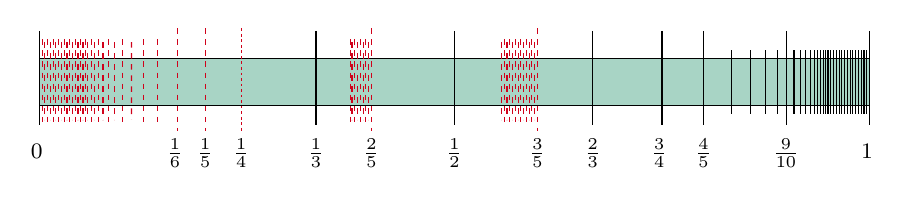
\begin{tikzpicture}[x=1pt,y=1pt,yscale=-1,xscale=1]
%uncomment if require: \path (0,300); %set diagram left start at 0, and has height of 300

%Shape: Rectangle [id:dp6031317002513319] 
\draw  [fill={rgb, 255:red, 82; green, 170; blue, 140 }  ,fill opacity=0.5 ]  (9,17) -- (309,17) -- (309,34) -- (9,34) -- cycle ;
%Straight Lines [id:da6093520074955262] 
\draw    (109,7) -- (109,41) ;
%Straight Lines [id:da5640723196233665] 
\draw    (159,7) -- (159,41) ;
%Straight Lines [id:da9515095927859913] 
\draw    (209,7) -- (209,41) ;
%Straight Lines [id:da36855815370263745] 
\draw    (234,7) -- (234,41) ;
%Straight Lines [id:da31526341903201416] 
\draw    (249,7) -- (249,41) ;
%Straight Lines [id:da6872953533879641] 
\draw    (279,7) -- (279,41) ;
%Straight Lines [id:da826511555809612] 
\draw [color={rgb, 255:red, 208; green, 2; blue, 27 }  ,draw opacity=1 ] [dash pattern={on 2pt off 2pt}]  (10,10) -- (10,40) ;
%Straight Lines [id:da826511555809612] 
\draw [color={rgb, 255:red, 208; green, 2; blue, 27 }  ,draw opacity=1 ] [dash pattern={on 2pt off 2pt}]  (11,11) -- (11,39) ;
%Straight Lines [id:da826511555809612] 
\draw [color={rgb, 255:red, 208; green, 2; blue, 27 }  ,draw opacity=1 ] [dash pattern={on 2pt off 2pt}]  (12,10) -- (12,40) ;
%Straight Lines [id:da826511555809612] 
\draw [color={rgb, 255:red, 208; green, 2; blue, 27 }  ,draw opacity=1 ] [dash pattern={on 2pt off 2pt}]  (13,11) -- (13,39) ;
%Straight Lines [id:da826511555809612] 
\draw [color={rgb, 255:red, 208; green, 2; blue, 27 }  ,draw opacity=1 ] [dash pattern={on 2pt off 2pt}]  (14,10) -- (14,40) ;
%Straight Lines [id:da826511555809612] 
\draw [color={rgb, 255:red, 208; green, 2; blue, 27 }  ,draw opacity=1 ] [dash pattern={on 2pt off 2pt}]  (15,11) -- (15,39) ;
%Straight Lines [id:da826511555809612] 
\draw [color={rgb, 255:red, 208; green, 2; blue, 27 }  ,draw opacity=1 ] [dash pattern={on 2pt off 2pt}]  (16,10) -- (16,40) ;
%Straight Lines [id:da826511555809612] 
\draw [color={rgb, 255:red, 208; green, 2; blue, 27 }  ,draw opacity=1 ] [dash pattern={on 2pt off 2pt}]  (17,11) -- (17,39) ;
%Straight Lines [id:da826511555809612] 
\draw [color={rgb, 255:red, 208; green, 2; blue, 27 }  ,draw opacity=1 ] [dash pattern={on 2pt off 2pt}]  (18,10) -- (18,40) ;
%Straight Lines [id:da826511555809612] 
\draw [color={rgb, 255:red, 208; green, 2; blue, 27 }  ,draw opacity=1 ] [dash pattern={on 2pt off 2pt}]  (19,11) -- (19,39) ;
%Straight Lines [id:da826511555809612] 
\draw [color={rgb, 255:red, 208; green, 2; blue, 27 }  ,draw opacity=1 ] [dash pattern={on 2pt off 2pt}]  (20,10) -- (20,40) ;
%Straight Lines [id:da826511555809612] 
\draw [color={rgb, 255:red, 208; green, 2; blue, 27 }  ,draw opacity=1 ] [dash pattern={on 2pt off 2pt}]  (21,11) -- (21,39) ;
%Straight Lines [id:da826511555809612] 
\draw [color={rgb, 255:red, 208; green, 2; blue, 27 }  ,draw opacity=1 ] [dash pattern={on 2pt off 2pt}]  (22,10) -- (22,40) ;
%Straight Lines [id:da826511555809612] 
\draw [color={rgb, 255:red, 208; green, 2; blue, 27 }  ,draw opacity=1 ] [dash pattern={on 2pt off 2pt}]  (23,11) -- (23,39) ;
%Straight Lines [id:da826511555809612] 
\draw [color={rgb, 255:red, 208; green, 2; blue, 27 }  ,draw opacity=1 ] [dash pattern={on 2pt off 2pt}]  (24,10) -- (24,40) ;
%Straight Lines [id:da826511555809612] 
\draw [color={rgb, 255:red, 208; green, 2; blue, 27 }  ,draw opacity=1 ] [dash pattern={on 2pt off 2pt}]  (24.79,11) -- (24.79,39) ;
%Straight Lines [id:da826511555809612] 
\draw [color={rgb, 255:red, 208; green, 2; blue, 27 }  ,draw opacity=1 ] [dash pattern={on 2pt off 2pt}]  (25.67,10) -- (25.67,40) ;
%Straight Lines [id:da826511555809612] 
\draw [color={rgb, 255:red, 208; green, 2; blue, 27 }  ,draw opacity=1 ] [dash pattern={on 2pt off 2pt}]  (26.5,11) -- (26.5,39) ;
%Straight Lines [id:da826511555809612] 
\draw [color={rgb, 255:red, 208; green, 2; blue, 27 }  ,draw opacity=1 ] [dash pattern={on 2pt off 2pt}]  (27.75,10) -- (27.75,40) ;
%Straight Lines [id:da826511555809612] 
\draw [color={rgb, 255:red, 208; green, 2; blue, 27 }  ,draw opacity=1 ] [dash pattern={on 2pt off 2pt}]  (29,11) -- (29,39) ;
%Straight Lines [id:da826511555809612] 
\draw [color={rgb, 255:red, 208; green, 2; blue, 27 }  ,draw opacity=1 ] [dash pattern={on 2pt off 2pt}]  (30.4,10) -- (30.4,40) ;
%Straight Lines [id:da826511555809612] 
\draw [color={rgb, 255:red, 208; green, 2; blue, 27 }  ,draw opacity=1 ] [dash pattern={on 2pt off 2pt}]  (32,11) -- (32,39) ;
%Straight Lines [id:da826511555809612] 
\draw [color={rgb, 255:red, 208; green, 2; blue, 27 }  ,draw opacity=1 ] [dash pattern={on 2pt off 2pt}]  (34,10) -- (34,40) ;
%Straight Lines [id:da826511555809612] 
\draw [color={rgb, 255:red, 208; green, 2; blue, 27 }  ,draw opacity=1 ] [dash pattern={on 2pt off 2pt}]  (36.27,11) -- (36.27,39) ;
%Straight Lines [id:da826511555809612] 
\draw [color={rgb, 255:red, 208; green, 2; blue, 27 }  ,draw opacity=1 ] [dash pattern={on 2pt off 2pt}]  (39,10) -- (39,40) ;
%Straight Lines [id:da4778652559233154] 
\draw [color={rgb, 255:red, 208; green, 2; blue, 27 }  ,draw opacity=1 ] [dash pattern={on 2pt off 2pt}]  (42.333,11) -- (42.33,39) ;
%Straight Lines 
\draw [color={rgb, 255:red, 208; green, 2; blue, 27 }  ,draw opacity=1 ] [dash pattern={on 2pt off 2pt}]  (46.5,10) -- (46.5,40) ;
%Straight Lines 
\draw [color={rgb, 255:red, 208; green, 2; blue, 27 }  ,draw opacity=1 ] [dash pattern={on 2pt off 2pt}]  (176,11) -- (176,39) ;
%Straight Lines 
\draw [color={rgb, 255:red, 208; green, 2; blue, 27 }  ,draw opacity=1 ] [dash pattern={on 2pt off 2pt}]  (177,10) -- (177,40) ;
%Straight Lines 
\draw [color={rgb, 255:red, 208; green, 2; blue, 27 }  ,draw opacity=1 ] [dash pattern={on 2pt off 2pt}]  (178,11) -- (178,39) ;
%Straight Lines 
\draw [color={rgb, 255:red, 208; green, 2; blue, 27 }  ,draw opacity=1 ] [dash pattern={on 2pt off 2pt}]  (179,10) -- (179,40) ;
%Straight Lines 
\draw [color={rgb, 255:red, 208; green, 2; blue, 27 }  ,draw opacity=1 ] [dash pattern={on 2pt off 2pt}]  (180,11) -- (180,39) ;
%Straight Lines 
\draw [color={rgb, 255:red, 208; green, 2; blue, 27 }  ,draw opacity=1 ] [dash pattern={on 2pt off 2pt}]  (181,10) -- (181,40) ;
%Straight Lines 
\draw [color={rgb, 255:red, 208; green, 2; blue, 27 }  ,draw opacity=1 ] [dash pattern={on 2pt off 2pt}]  (182,11) -- (182,39) ;
%Straight Lines 
\draw [color={rgb, 255:red, 208; green, 2; blue, 27 }  ,draw opacity=1 ] [dash pattern={on 2pt off 2pt}]  (183,10) -- (183,40) ;
%Straight Lines 
\draw [color={rgb, 255:red, 208; green, 2; blue, 27 }  ,draw opacity=1 ] [dash pattern={on 2pt off 2pt}]  (184,11) -- (184,39) ;
%Straight Lines 
\draw [color={rgb, 255:red, 208; green, 2; blue, 27 }  ,draw opacity=1 ] [dash pattern={on 2pt off 2pt}]  (185,10) -- (185,40) ;
%Straight Lines 
\draw [color={rgb, 255:red, 208; green, 2; blue, 27 }  ,draw opacity=1 ] [dash pattern={on 2pt off 2pt}]  (186,11) -- (186,39) ;
%Straight Lines 
\draw [color={rgb, 255:red, 208; green, 2; blue, 27 }  ,draw opacity=1 ] [dash pattern={on 2pt off 2pt}]  (187,10) -- (187,40) ;
%Straight Lines 
\draw [color={rgb, 255:red, 208; green, 2; blue, 27 }  ,draw opacity=1 ] [dash pattern={on 2pt off 2pt}]  (188,11) -- (188,39) ;
%Straight Lines 
\draw [color={rgb, 255:red, 208; green, 2; blue, 27 }  ,draw opacity=1 ] [dash pattern={on 2pt off 2pt}]  (121.5,10) -- (121.5,40) ;
%Straight Lines 
\draw [color={rgb, 255:red, 208; green, 2; blue, 27 }  ,draw opacity=1 ] [dash pattern={on 2pt off 2pt}]  (122,11) -- (122,39) ;
%Straight Lines 
\draw [color={rgb, 255:red, 208; green, 2; blue, 27 }  ,draw opacity=1 ] [dash pattern={on 2pt off 2pt}]  (123,10) -- (123,40) ;
%Straight Lines 
\draw [color={rgb, 255:red, 208; green, 2; blue, 27 }  ,draw opacity=1 ] [dash pattern={on 2pt off 2pt}]  (124,11) -- (124,39) ;
%Straight Lines 
\draw [color={rgb, 255:red, 208; green, 2; blue, 27 }  ,draw opacity=1 ] [dash pattern={on 2pt off 2pt}]  (125,10) -- (125,40) ;
%Straight Lines 
\draw [color={rgb, 255:red, 208; green, 2; blue, 27 }  ,draw opacity=1 ] [dash pattern={on 2pt off 2pt}]  (126,11) -- (126,39) ;
%Straight Lines 
\draw [color={rgb, 255:red, 208; green, 2; blue, 27 }  ,draw opacity=1 ] [dash pattern={on 2pt off 2pt}]  (127,10) -- (127,40) ;
%Straight Lines 
\draw [color={rgb, 255:red, 208; green, 2; blue, 27 }  ,draw opacity=1 ] [dash pattern={on 2pt off 2pt}]  (128,11) -- (128,39) ;
%Straight Lines 
\draw [color={rgb, 255:red, 208; green, 2; blue, 27 }  ,draw opacity=1 ] [dash pattern={on 2pt off 2pt}]  (51.857,10) -- (51.857,40) ;
%Straight Lines [id:da31637779955599454] 
\draw [color={rgb, 255:red, 208; green, 2; blue, 27 }  ,draw opacity=1 ] [dash pattern={on 2pt off 2pt}]  (59,6) -- (59,43) ;
%Straight Lines [id:da4498884699950627] 
\draw [color={rgb, 255:red, 208; green, 2; blue, 27 }  ,draw opacity=1 ] [dash pattern={on 2pt off 2pt}]  (69,6) -- (69,43) ;
%Straight Lines [id:da18401946654000256] 
\draw [color={rgb, 255:red, 208; green, 2; blue, 27 }  ,draw opacity=1 ] [dash pattern={on 1pt off 1pt}]  (82,6) -- (82,43) ;
%Straight Lines [id:da5280544755627746] 
\draw [color={rgb, 255:red, 208; green, 2; blue, 27 }  ,draw opacity=1 ] [dash pattern={on 2pt off 2pt}]  (129,6) -- (129,43) ;
%Straight Lines [id:da4333895960809735] 
\draw [color={rgb, 255:red, 208; green, 2; blue, 27 }  ,draw opacity=1 ] [dash pattern={on 2pt off 2pt}]  (189,6) -- (189,43) ;
%Straight Lines [id:da2422812299045457] 
\draw    (9,7) -- (9,41) ;
%Straight Lines [id:da5995861597296466] 
\draw    (309,7) -- (309,41) ;
%Straight Lines [id:da6493611634458583] 
\draw    (294,14) -- (294,37) ;
%Straight Lines 
\draw    (266.14,14) -- (266.14,37) ;
%Straight Lines 
\draw    (271.5,14) -- (271.5,37) ;
%Straight Lines 
\draw    (275.67,14) -- (275.67,37) ;
%Straight Lines 
\draw    (281.727,14) -- (281.727,37) ;
%Straight Lines 
\draw    (284,14) -- (284,37) ;
%Straight Lines 
\draw    (286,14) -- (286,37) ;
%Straight Lines 
\draw    (287.57,14) -- (287.57,37) ;
%Straight Lines 
\draw    (291.353,14) -- (291.353,37) ;
%Straight Lines 
\draw    (292.333,14) -- (292.333,37) ;
%Straight Lines 
\draw    (290.25,14) -- (290.25,37) ;
%Straight Lines 
\draw    (259,14) -- (259,37) ;
%Straight Lines [id:da35077934027273827] 
\draw    (271.5,14) -- (271.5,37) ;
%Straight Lines [id:da15302073574897146] 
\draw    (289,14) -- (289,37) ;
%Straight Lines [id:da26639239361194333] 
\draw    (304,14) -- (304,37) ;
%Straight Lines [id:da9353856632014482] 
\draw    (300,14) -- (300,37) ;
%Straight Lines 
\draw    (293,14) -- (293,37) ;
%Straight Lines 
\draw    (294,14) -- (294,37) ;
%Straight Lines 
\draw    (295,14) -- (295,37) ;
%Straight Lines 
\draw    (296,14) -- (296,37) ;
%Straight Lines 
\draw    (297,14) -- (297,37) ;
%Straight Lines 
\draw    (298,14) -- (298,37) ;
%Straight Lines 
\draw    (299,14) -- (299,37) ;
%Straight Lines 
\draw    (300,14) -- (300,37) ;
%Straight Lines 
\draw    (301,14) -- (301,37) ;
%Straight Lines 
\draw    (302,14) -- (302,37) ;
%Straight Lines 
\draw    (303,14) -- (303,37) ;
%Straight Lines 
\draw    (304,14) -- (304,37) ;
%Straight Lines 
\draw    (305,14) -- (305,37) ;
%Straight Lines 
\draw    (306,14) -- (306,37) ;
%Straight Lines 
\draw    (307,14) -- (307,37) ;
%Straight Lines 
\draw    (308,14) -- (308,37) ;

% Text Node
\draw (54,45) node [anchor=north west][inner sep=0.75pt]  [font=\footnotesize]  {$\frac{1}{6}$};
% Text Node
\draw (65,45) node [anchor=north west][inner sep=0.75pt]  [font=\footnotesize]  {$\frac{1}{5}$};
% Text Node
\draw (78,45) node [anchor=north west][inner sep=0.75pt]  [font=\footnotesize]  {$\frac{1}{4}$};
% Text Node
\draw (105,45) node [anchor=north west][inner sep=0.75pt]  [font=\footnotesize]  {$\frac{1}{3}$};
% Text Node
\draw (155,45) node [anchor=north west][inner sep=0.75pt]  [font=\footnotesize]  {$\frac{1}{2}$};
% Text Node
\draw (125,45) node [anchor=north west][inner sep=0.75pt]  [font=\footnotesize]  {$\frac{2}{5}$};
% Text Node
\draw (185,45) node [anchor=north west][inner sep=0.75pt]  [font=\footnotesize]  {$\frac{3}{5}$};
% Text Node
\draw (205,45) node [anchor=north west][inner sep=0.75pt]  [font=\footnotesize]  {$\frac{2}{3}$};
% Text Node
\draw (229,45) node [anchor=north west][inner sep=0.75pt]  [font=\footnotesize]  {$\frac{3}{4}$};
% Text Node
\draw (245,45) node [anchor=north west][inner sep=0.75pt]  [font=\footnotesize]  {$\frac{4}{5}$};
% Text Node
\draw (273,45) node [anchor=north west][inner sep=0.75pt]  [font=\footnotesize]  {$\frac{9}{10}$};
% Text Node
\draw (305,47) node [anchor=north west][inner sep=0.75pt]  [font=\footnotesize]  {$1$};
% Text Node
\draw (5,47) node [anchor=north west][inner sep=0.75pt]  [font=\footnotesize]  {$0$};


\end{tikzpicture}

    \caption{Quantile-wise tractability or intractability of max \ESW{}. Red dashed lines show values of $\tau$ for which maximizing \ESW{} is NP-hard, black solid lines show a value for $\tau$ for which we have polytime algorithms.}
    \label{fig:ESWpvsnp}
\end{figure*}
\subsection{Egalitarian Social Welfare}
Rather surprisingly, we  find that maximizing \ESW{} over all allocations is intractable for some quantiles and tractable for others. Here, we assume all agents have the same quantiles. Clearly, the intractability results would extend to settings with arbitrary heterogeneous valuations.  We illustrate the spectrum of quantiles for which the problem is tractable vs intractable in \cref{fig:ESWpvsnp}. 
When presenting algorithms, we shall again assume binary valuations. From \cref{lem:binRednESW}, a polynomial time algorithm for the binary case is sufficient to get a general algorithm.

\subsubsection{Exact Algorithms. } We are able to find polynomial time algorithms for maximizing \ESW{} under a class of quantiles which includes many natural quantiles like $\tau = 0,\sfrac{1}{2},\sfrac{2}{3},\sfrac{3}{4},\sfrac{9}{10}$. 
We begin with a simple observation which is true for all quantiles: it must be possible to simultaneously allocate at least one item of value $1$ to each agent. 


\begin{observation}\label{obs:egalbasic}
    Under an instance with binary goods, for allocation $A$, $\ESW{}(A)=1$ if and only if for each $i\in N$, there exists $g\in A_i$, s.t. $v_i(g)=1$.
\end{observation}

This gives a necessary condition for an allocation with \ESW{} of 1 to exist.  We now specifically consider quantiles of the form $\tau=\frac{t}{t+1}$ for $k\in \mathbb{Z}_+$. For this setting, we have the following simple result.

\begin{restatable}{lemma}{toffset}\label{lem:eswhalf}
    For an agent $i\in N$ with $\tau_i=\frac{t}{t+1}$, where $t\in \mathbb{Z}_+$ is fixed, a bundle $B\subseteq M$ with exactly $\ell$ goods of value $1$ for $i$, we have that $v_i(B)=1$ if and only if the number of 0 valued items in $B$ for $i$ is at most $\ell t-1$. 
\end{restatable}

\begin{proof}
    
    Given agent $i$ and bundle $B$ with exactly $\ell$ goods of value $1$ for $i$. Observe that it is sufficient to compare the case when there are either exactly $\ell  t-1$ items of value $0$ or $\ell t$ items of value $0.$
    
    Suppose the number of items of value $0$ is $\ell t$. The value of agent $i$ for $B$ would be from  the $\lceil (\ell t+\ell)\frac{t}{t+1}\rceil =\ell t$'th lowest valued item, which would have value $0$. Consequently $v_i(B)=0$.

    On the other hand, if $B$ contained  $\ell t-1$ items of value $0$, then $i$'s value would come from the item which has the $p$th lowest value where  

    \begin{align*}
        p &= \Bigl\lceil (\ell t-1+\ell)\frac{t}{t+1}\Bigr\rceil\\
          &= \Bigl\lceil\frac{\ell t^2+\ell t-t}{t+1}\Bigr\rceil \\
          &=\Bigl\lceil (\ell t- \frac{t}{t+1})\Bigr\rceil \\
          &= \ell t \tag{As $\frac{t}{t+1}<1$.}
    \end{align*}
    
    %\haris{end equations with a period}
    As a result, when there are at most $\ell t-1$ items of value $0$, $v_i(B)=1$.
\end{proof}

Based on \cref{obs:egalbasic} and \cref{lem:eswhalf} we develop an algorithm for maximizing \ESW{} over unbalanced allocations when there is a $t\in \mathbb{Z}_+$ s.t. $\tau_i=\frac{t}{t+1}$ for each $i\in N$. We divide the items into two set $M_0$ and $M_1$. Items in $M_0$ are objective $0$s, that is, all agents have value $0$ for each item in $M_0$. The remaining items are in $M_1$ which are subjective $1$s. That is, these are the items for which at least $1$ agent who has value $1$. 

The algorithm checks for two conditions: are there enough items so that each agent can receive a good of value $1$ and are there enough items in $M_1$ to offset the items in $M_0$. If so, it first assigns each agent an item they have value $1$ for. Next, out of the unassigned items in $M_1$, it arbitrarily selects one such item and allocates it to an agent who has value $1$ for it, along with $t$ items from $M_0$. Finally, if no items remain in one of $M_0$ or $M_1$, it allocates the remaining items while ensuring the condition in \cref{lem:eswhalf}.  

%\haris{It will be nice to have informal descriptions of the algos outside the proof environment}

{
\begin{algorithm}[t]
  \KwIn{$I=\langle N,M, v,\tau \rangle$ with binary goods and $\tau=\sfrac{t}{t+1}$ }
  \KwOut{An allocation $A$}
    Create bipartite graph $G=(X,Y,E)$ where $X$ contains $x_g$ for each $g\in M$,
    $Y$ contains $y_i$ for each $i\in N$ and 
    $(x_g,y_i)\in E$ only if $v_i(g)=1$, for each $i\in N,\, g\in M$\;
    Let $\mu$ be a maximum cardinality matching in $G$\; 
    %
    Let $M_0=\{g\in M|v_i(g)=0$ for all $i\in N\}$\;
    Let $M_1=M\setminus M_0$\;\label{step:defn} 
    \eIf{$|M_0|> t|M_1|-n$ OR $|\mu|<n$}{
        Let $A$ be an arbitrary allocation\;
    }
    {
        Let $A=(A_1,\cdots, A_n)$ be s.t. $A_i\gets\{g|(x_g,y_i)\in \mu\}$\;\label{step:else}
        $M_1\gets M_1\setminus \cup_i A_i$\;
        \While{$M_1\neq \emptyset$ AND $M_0\neq \emptyset$}{
            Arbitrarily pick $g\in M_1$ and $i\in N$ s.t. $v_i(g)=1$\;
            \eIf{$|M_0|\geq t$}{
                Pick an arbitrary subset $S\subseteq M_0$ s.t. $|S|=t$\;
            }{
                Let $S\gets M_0$\;
            }
            $A_i\gets A_i\cup \{g\}\cup S$\;
            $M_1\gets M_1\setminus \{g\}$ and 
            $M_0\gets M_0 \setminus S$\;
        }
        \If{$M_0\neq \emptyset$}{
            Let $B_1\cdots B_n$ be an arbitrary partition of $M_0$ s.t. $|B_i|\leq t-1$ for all $i\in N$\;
            
        }
        \If{$M_1\neq \emptyset$}{
            Let $B_1\cdots B_n$ be an arbitrary partition of $M_1$ s.t. $g\in|B_i|$ only if $v_i(g)=1$\;
        }
        For each $i\in N$, set $A_i\gets A_i \cup B_i$\;
      
    }
    \textbf{Return} $A$\;    
        
   \caption{Max \ESW{} for binary goods and $\tau=\sfrac{t}{t+1}$}\label{alg:ESW-unbal}
\end{algorithm}
}

\begin{restatable}{proposition}{ESWunbal}\label{prop:ESWunbal}
    Given instance $I=\langle N,M,v,\tau=\frac{t}{t+1}\rangle$ where $t\in \mathbb{Z}_+$, \cref{alg:ESW-unbal} returns a maximum \ESW{} allocation in polynomial time.
\end{restatable}


\begin{proof}
    We now show that given an instance with binary goods $I=\langle N,M,v, \tau=\frac{t}{t+1}\rangle$, \cref{alg:ESW-unbal} finds an allocation with \ESW{} of $1$ whenever it exists.  

    Let $\mu$, $M_0$ and $M_1$ be as defined in \cref{alg:ESW-unbal} by step \ref{step:defn}.  We shall now show that whenever an allocation of \ESW{} $1$ exists, \cref{alg:ESW-unbal} will return an allocation with \ESW{} $1$. We first show that when $|\mu|=n$ and $|M_0|\leq t|M_1|-n$, \cref{alg:ESW-unbal} creates an allocation where if agent $i\in N$ receives $\ell_i>1$ items of value $1$ then they receive at most $t\ell_i-1$ items of value $0$. We have that $\ell _i>1$ as $\mu$ matches each agent to an item of value $1$. 
    
    Further, in the while loop, whenever $i$ receives at most $t$ $0$ valued items from $M_0$, they are accompanied with one item of value $1$. After the while loop, an additional $t-1$ items of value $0$ may be  allocated to $i$. As a result, $v_i(A_i)=1$ in this case.

    Consequently, when $|\mu|=n$ and $|M_0|\leq t|M_1|-n$, we have that \cref{alg:ESW-unbal} finds an allocation with $\ESW{}(A)=1$.

    Conversely, assume that an allocation $A^*$ exists s.t. $\ESW{}(A^*)=1$. Now, clearly each agent $i$ must receive at least one good of value $1$, thus we have that $|\mu|=n$. 

    Now let $A^*_{i,0}$ and $A^*_{i,1}$ respectively denote the $0$ and $1$ valued items $i$ is allocated under $A^*$. We have that $M_0\subseteq \cup_{i\in N} A^*_{i,0}$ and $\cup_{i\in N} A^*_{i,1}\leq M_1$. 

    As $v_i(A^*_i)=1$, from \cref{lem:eswhalf}, we have that $|A_{i,0}^*|\leq t|A^*_{i,1}|-1$. Consequently, we have that 
    \[|M_0|\leq \sum_i |A_{i,0}^*|\leq \sum_i t|A^*_{i,1}|-1\leq t|M_1| - n  \]

    Hence, we have that the necessary conditions will be satisfied and \cref{alg:ESW-unbal} will return an allocation of \ESW{} $1$. As a result, \cref{alg:ESW-unbal} will return an allocation with \ESW{} $1$ if and only if one exists.
\end{proof}

We now extend this idea to the setting of $\tau_i=\sfrac{1}{3}$ for all agents. Here, we begin with the following simple observation, analogous to \cref{lem:eswhalf}.

\begin{observation}\label{obs:third}
    For an agent $i\in N$ with $\tau_i=\sfrac{1}{3}$, a bundle $B\subseteq M$ with exactly $\ell $ items of value $0$ for $i$, we have that $v_i(B)=1$ if and only if the number of $1$ valued items in $B$ is at least $2\ell +1$.
\end{observation}
    
\iffalse

\begin{proof}
    %Given an agent $i$ with $\tau_i=\sfrac{1}{3}$ and a bundle $B\subseteq M$ s.t. $B$ with exactly $d$ items of value $0$. 
    
    Observe that it is enough to consider the case when the number of $1$ valued items is either $2\ell $ or $2\ell $.

    Let $B$ have $2\ell $ items of value $1$. Consequently, the value of $B$ will come from the $\lceil (\ell +2\ell )\frac{1}{3}\rceil = \ell $th item. As a a result, $v_i(B)=0$.

    Now let $B$ have $2\ell +1$ items of value $1$. The value of $B$ will come from the $\lceil (3d+1)\frac{1}{3}\rceil=d+1$th item. Consequently, $v_i(B)=1$.

    Hence, $v_i(B)=1$ if and only if there are at least $2\ell +1$ items of value $1$.
\end{proof}
\fi

Thus, when $M_0$ and $M_1$ are as in \cref{alg:ESW-unbal}, we need two items from $M_1$ to offset one from $M_0$. We can now build \cref{alg:ESW-unbalthird} where we need to check if we can satisfy both \cref{obs:egalbasic,obs:third}. 



\begin{algorithm}[t]
  \KwIn{$I=\langle N,M, v,\tau \rangle$ with binary goods and $\tau=\sfrac{1}{3}$ }
  \KwOut{An allocation $A$}
    Let $M_0=\{g\in M|v_i(g)=0$ for all $i\in N\}$\;
    Let $M_1=M\setminus M_0$\;
    Create graph $G=(X \cup Y, E)$ where $X$ contains $x_g$ for each $g\in M_1$, 
    $Y$ contains $y_i$ for each $i\in N$ and $(x_g,y_i)\in E$ only if $v_i(g)=1$ and 
    $(x_g,x_{g'})\in E$ only if there exists $i\in N$ s.t. $v_i(g)=v_i(g')=1$\;
    Define edge weight function $w$ where $w(x,y)=|X\cup Y|+1$ and $w(y,y')=1$\;
    Let $\mu$ be a maximum weight matching in $G_2$\; %\label{step:defn} 
    
    \eIf{$w(\mu)<|M_0|+n(|X\cup Y|+1)$}{
        Let $A$ be an arbitrary allocation\;
    }
    {
        Let $A=(A_1,\cdots, A_n)$ be such that $A_i=\{g|(x_g,y_i)\in \mu\}$\;%\label{step:else}
        $M_1\gets M_1\setminus \cup_i A_i$\;
        \While{$M_0\neq \emptyset$}{
            Arbitrarily pick $g_0\in M_0$ and $g,g'$ s.t. $(x_{g},x_{g'})\in \mu$\;
            Pick $i\in N$ s.t. $v_i(g)=v_i(g')=1$\; 
            $A_i\gets A_i\cup \{g_0,g,g'\}$\;
            $M_1\gets M_1\setminus \{g,g'\}$ and 
            $M_0\gets M_0 \setminus \{g_0\}$\;
        }
        \If{$M_1\neq \emptyset$}{
            Let $B_1\cdots B_n$ be an arbitrary partition of $M_1$ s.t. $g\in|B_i|$ only if $v_i(g)=1$\;
        }
        For each $i\in N$, set $A_i\gets A_i \cup B_i$\;
        
    }
    \textbf{Return} $A$\;    
        
   \caption{Max \ESW{} binary goods for $\tau=\sfrac{1}{3}$}\label{alg:ESW-unbalthird}
\end{algorithm}


\begin{restatable}{proposition}{ESWunbalthird}\label{prop:ESWunbalthird}
    Given $I=\langle N,M,v,\tau=\sfrac{1}{3}\rangle$, \cref{alg:ESW-unbalthird} returns a maximum \ESW{} allocation in polynomial time.
\end{restatable}


\begin{proof}
    We now show that given an instance with binary goods $I=\langle N,M,v, \tau=\sfrac{1}{3}\rangle$, \cref{alg:ESW-unbalthird} finds an allocation with \ESW{} of $1$ whenever it exists.  

    Let $\mu$ $M_0$ and $M_1$ be as initially defined in \cref{alg:ESW-unbalthird}.  We shall now show that whenever an allocation of \ESW{} $1$ exists, \cref{alg:ESW-unbal} will return an allocation with \ESW{} $1$. We first show that when $w(\mu)\geq|M_0|+n(|X\cup Y|+1)$, \cref{alg:ESW-unbalthird} creates an allocation where if agent $i\in N$ receives $\ell_i$ items of value $0$, then they receive at least $2\ell_i+1$ items of value $1$. 

    Firstly, $\mu$ matches each agent to one item of value $1$, so for agents with $\ell_i=0$, the requirement is satisfied.     
    Further, in the while loop, whenever $i$ receives two items of value $1$ for every item from $M_0$. After the while loop,  only items of value $1$ may be  allocated to $i$. As a result, $v_i(A_i)=1$ in this case.

    Consequently, when $w(\mu)\geq|M_0|+n(|X\cup Y|+1)$, we have that \cref{alg:ESW-unbalthird} finds an allocation with $\ESW{}(A)=1$.

    Conversely, assume that an allocation $A^*$ exists s.t. $\ESW{}(A^*)=1$. %Now, clearly each agent $i$ must receive at least one good of value $1$, thus we have that $|\mu|>=n$. 
%
    Now let $A^*_{i,0}$ and $A^*_{i,1}$ respectively denote the $0$ and $1$ valued items $i$ is allocated under $A^*$. We have that $M_0\subseteq \cup_{i\in N} A^*_{i,0}$ and $\cup_{i\in N} A^*_{i,1}\leq M_1$. 

    As $v_i(A^*_i)=1$, from \cref{lem:eswhalf}, we have that $|A_{i,1}^*|\geq 2|A^*_{i,0}|+1$. Consequently, we have can build a matching $\mu'$ in in $G_2$ matching $|A^*_{i,0}|$ pairs of items from $A^*_{i,1}$ to each other and one additional item to $i$. Now as $\mu_2$ is a maximum weight matching in $G_2$, it must have weight at least  
    \begin{align*}
        w(\mu_2) &\geq w(\mu')\\
                 &\geq \sum_i (|A^*_{i,0}| +  |X\cup Y|+1)\\
                 &= n(|X\cup Y|+1)+\sum_i |A^*_{i,0}| \\
                 &\geq  n(|X\cup Y|+1)+|M_0|.
    \end{align*}

    Hence, we have that the necessary condition will be satisfied and \cref{alg:ESW-unbal} will return an allocation of \ESW{} $1$. As a result, \cref{alg:ESW-unbal} will return an allocation with \ESW{} $1$ if and only if one exists.
\end{proof}



We can now summarize our tractability results for maximum \ESW{} over all allocations as follows. 

\begin{theorem}\label{thm:ESWunbal}
    A maximum \ESW{} allocation can be found in polynomial time for $\tau=\{0,\sfrac{1}{3},1\}\cup \{\frac{t}{t+1}|t\in \mathbb{Z}_+\}$.
\end{theorem}


\subsubsection{Intractability.} We now show that there are several quantile values for which maximizing \ESW{} is NP-hard. Intriguingly, these values interweave between quantile values for which maximizing \ESW{} can be done in polynomial time. We find three ranges of intractability. Namely, for $\tau\in \{\sfrac{1}{t}|t\geq 4\}\cup (\sfrac{3}{8},\sfrac{2}{5}]\cup (\sfrac{5}{9},\sfrac{3}{5}]$. For $\tau=\sfrac{1}{t}$ where $t\geq 4$, one item of value $0$ needs to be offset by $t$ items of value $1$. We show that this can be equivalent to a $t-1$ dimensional matching. 
For $\tau\in (\sfrac{3}{8},\sfrac{2}{5}]$ or $\tau\in (\sfrac{5}{9},\sfrac{3}{5})$ the ratio of additional items of value $1$ for a new item of value $0$ can vary. We find that deciding between these cases proves to be NP-hard. %we have that depending on the context, there are times when one item of value $0$ needs two items of value $1$ to offset it and at other times, only item of value $1$ is needed. Deciding between these proves to be intractable. In a similar vein, when  there are bundles where an additional item of value $1$ can offset two new items of value $0$. For other bundles, one items of value $1$ can offset only one item of value $0.$ 
In all three cases, we prove NP-hardness via a reduction from \textup{\textsc{Exact3Cover}}.

\begin{theorem}\label{thm:ESWunbalNP}
    Given $I=\langle N,M,v,\tau\rangle$, maximizing \ESW{} is NP-hard for $\tau\in \{\sfrac{1}{t}|t\geq 4\}\cup (\sfrac{3}{8},\sfrac{2}{5}]\cup (\sfrac{5}{9},\sfrac{3}{5}]$.
\end{theorem}
%\begin{corollary}
%    For binary goods, finding a max $\USW{}$ allocation is NP-hard to $\tau=\sfrac{1}{4}$ or $\sfrac{2}{5}$.
%\end{corollary}






%%%%%%%%%%%%%%%%%%%%%%%%%%%%%%%%%%%%%%%%%%%%%%%%%%%%%%%%%%%%%%%%
%%%%%%%%%%%%%%%%%%%%%%%%%%%%%%%%%%%%%%%%%%%%%%%%%%%%%%%%%%%%%%%%
%%%%%%%%%%%%%%%%%%%%%%%%%%%%%%%%%%%%%%%%%%%%%%%%%%%%%%%%%%%%%%%% 
\section{Chores}

We now turn our attention to the case of {\em chores}. Here, all items give all agents non-positive values. Recall that for chores, we capture agent preferences via {\em disutilities} and aim to minimize utilitarian and egalitarian social {\em costs}. 

%The results for balanced allocations with goods extend in a straightforward manner to the case of chores. In fact, \cref{alg:balESW} extends to settings with mixed goods and chores. Consequently, in this section we focus entirely on {\em minimizing} utilitarian and egalitarian social {\em cost} without the balancedness requirement.

\subsection{Utilitarian Social Cost}\label{sec:USCchores}

\paragraph{Balanced Allocations. } Under balanced allocations, we had seen in \cref{subsec:balUSW} that maximum \USW{} is hard to approximate. While the same reduction does not extend well to the case, of chores, it can be seen from a simple reduction from \textup{\textsc{Exact3Cover}} (X3C) that the problem is NP-hard. Similarly, while the greedy algorithm (\cref{alg:goods-USWbalanced}) can be arbitrarily bad for chores, a minimum \ESC{} allocation (which we shall discuss in \cref{sec:ESCchores}) can be shown to be at most $\USC{ \max_{i\in N,\, g\in M} d_i(g)}$.
 
\paragraph{Unbalanced Allocations}. While goods allow for a near exact algorithm, for chores, one is not possible. We now show that minimizing \USC{} when all agents quantiles is $0$, is equivalent to the \textup{\textsc{WeightedSetCover}} problem.  This enables us to show that with chores and pessimistic agents (quantile $\tau=0$) no polytime algorithm can guarantee better than $\log m$ approximation to minimum  $\USC{}$, unless $P=NP$. 

\begin{restatable}{theorem}{apxusc}\label{thm:APX-USC}
    Given instance $I=\langle N, M, d,\tau=0 \rangle$ with chores, it is NP-hard to find an \USC{$(1-o(1))\log m$} allocation.% for any constant $c>0$. %\haris{indicate the restrictions and conditions for the hardness result: what quantile etc.}
\end{restatable}


Given an instance with chores, $I=\langle N, M, d,\tau=0 \rangle$, we can get an analogous reduction to weighted set cover. Here we construct an element for each item and a set for each agent and each disutility level. That is, for each agent, we create a set with top top $k$ best chores, for each $k\in [m]$. The corresponding weight of the set will be the agent's disutility for the set. We can now see that there is a mapping between set covers of weight at most $\nu$ and to allocations of \USC{} at most $\nu$. Thus, the $\log m$-approximation algorithm for weighted set cover provides a $\USC{\log m}$ algorithm for pessimistic agents. 

\subsection{Egalitarian Social Cost}\label{sec:ESCchores}

We had begun our exploration of egalitarian welfare in \cref{lem:binRednESW}, by showing that for goods, it is sufficient to find algorithms for binary goods. We can get an analogous result for the case of egalitarian cost. 

\begin{lemma}\label{lem:binRednChores}
The problem of finding an allocation with \ESC{} at most $\nu\geq0$ over allocations in $\Pi'\subseteq \Pi(n,M)$ under  heterogeneous quantiles reduces to the problem of minimizing \ESC{} over $\Pi'$ under binary chores with heterogeneous quantiles. 
\end{lemma}

We can now focus our discussion on binary chores where $d_i(g)\in \{0,1\}$ for all $i\in N$ and all $g\in M$. For balanced allocations, it is straightforward to see that the ideas for binary goods for {\em balanced allocations} extend to binary chores. Recall \cref{alg:balESW}. Instead of adding edges for items of value $1$, we add an edge for chores for disutility $0$. The result will then analogously follow.  

\begin{theorem}
    Given an instance with chores and heterogeneous quantiles $I=\langle N,M,d,\tau\rangle$ where $m=kn$, a minimum \ESC{} balanced allocation can be found in polynomial time.  
\end{theorem}

\paragraph{Unbalanced Allocations. } Recall that for goods, the tractability of egalitarian welfare was highly quantile dependent. \cref{alg:ESW-unbal} found a maximum \ESW{} allocation in polynomial time for quantiles of the form $\tau=\sfrac{t}{t+1}$ for $t\in \mathbb{Z^+}$. We now show that for chores, not only does \cref{alg:ESW-unbal} not extend, but the corresponding quantiles prove to be NP-hard. 

\begin{restatable}{theorem}{ESChalfNP}\label{thm:ESChalfNP}
    Given an instance $I=\langle N,M,d,\tau=\sfrac{1}{2}\rangle$, finding a minimum \ESC{} allocation is NP-hard.
\end{restatable}


\paragraph{Exact Algorithms.} In this manner, most of the quantiles for which we had exact algorithms for goods become intractable. For two specific quantiles however, we continue to have simple exact algorithms: $\tau=0$ and $\tau=1$. If $\tau=0$, it is sufficient to check for the given binary chores instance, if there is an item that is a universal bad, in which case all allocations will have \ESC{} of 1. If not, each item has at least one agent who has no disutility for it, and can be arbitrarily assigned to such an agent to get an allocation with \ESC{} of $0$. For $\tau=1$, if any one agent has even item with no disutility, they can be given all the items in $M$ to get an allocation with \ESC{} of $0$. Otherwise, each allocation must have \ESC{} of $1$. 

\section{Conclusions}
In this work,  we proposed a novel quantile-based preference model  in the context of indivisible item allocation.
 We studied {\em Utilitarian} and {\em Egalitarian Welfare}, both with and without the balanced allocation requirement, and provided comprehensive algorithmic and complexity-theoretic results.
  
  Interestingly, our results reveal that the complexity of the problems changes significantly depending on whether the balancedness requirement is imposed. For instance, for  balanced allocations there is a strong hardness of approximation bound for maximizing USW, whereas without the balancedness requirement, a near-exact approximation algorithm exists.  A similar phenomenon occurs with  \ESW{} but in reverse: for balanced allocations, maximizing \ESW{} can be solved efficiently, while without the balancedness requirement, maximizing \ESW{} is NP-hard  for many quantile values.

  Our work opens up several promising directions for future research. Firstly, while we focused on the two extremes of the p-means (Utilitarian and Egalitarian welfare), exploring other welfare functions, such as Nash welfare, presents an intriguing avenue for study. Secondly, investigating the compatibility between fairness notions, such as EF1 or EFx, and Pareto efficiency within the framework of our valuation class is another interesting direction of further research. 

\section*{Acknowledgements}

Haris Aziz and Shivika Narang are supported by the NSF-CSIRO project on “Fair Sequential Collective Decision-Making”. Mashbat Suzuki is supported by the ARC Laureate Project FL200100204 on “Trustworthy AI”.

\bibliographystyle{abbrvnat}
\bibliography{references.bib}

%
\clearpage
\appendix
\section{Additional Related Work}\label{app:relwork}

\paragraph{Allocating Indivisible Items.} The problem of allocating indivisible items fairly and/or efficiently is very well studied (See \cite{AAB+2022fair} for a survey). Existing literature almost exclusively assumes that preferences are aggregated in a monotone manner, often assuming additive valuations \citep{CKM+2019unreasonable,ACIW2022fair}, but also at times subadditive \citep{BKKN2024sublinear,BCIZ2020finding}  or superadditive valuations \citep{BVV2023fair,ViZi2023weighted}. A couple of papers also consider arbitrary valuations, with no underlying structure guaranteed, in addition to monotone valuations \citep{BBB+2024envy,BBPP2024nearly}. Our paper considers quantile preferences which may be monotone for the two extreme  quantiles, but non-monotone for all others.  

While typical work on allocating indivisible items does not explicitly restrict the type of allocations studied there has been some work restricting the number of items that can be allocated. \citet{SHS2023efficient} and \cite{BiBa2018fair} consider a setting where items are partitioned into categories and there is a uniform constraint on how many items of each category can be allocated to a single agent. For this space, \citet{BiBa2018fair} focus on envy based fairness, while \citet{SHS2023efficient} consider efficiency via pareto optimality and envy-based fairness. 

\citet{CaNa2024repeatedly} study a repeated matching setting where there are $T$ rounds and $n$ agents and $n$ items. In each round, each agent must receive exactly one item. Here, value for an item depends on how many times this agent has received the item in the past. For this space, \cite{CaNa2024repeatedly} pursue utilitarian social welfare and envy-based fairness.

 \paragraph{Quantile based preferences. } Quantile based preferences are well-established in mathematical economics and social choice theory. \cite{DeGa2019dynamic,DeGa2022static} show that quantile preferences are a more accurate model of real-life behavior of agents in random settings over expected utility. 
 
 These preferences are a generalization of \textit{preference set extensions} that lift preferences over individual items to a set of items. The study of preference set extensions has a long-standing history in social choice theory~\citep{BBP04a} and has been applied to hedonic coalition formation games~\citep{CeHa2003computational,CeHa2004stable,Cech08a}, committee selection~\citep{AzMo20a} and multidimensional matchings \citep{HNR2025strategyproof}. Among them, one is called the \textit{best set extension} in which the sets are compared based on the best item in each set. One is called the \textit{worst set extension},   in which the sets are compared based on the best item in each set. The best and worst extension correspond to the $\tau=1$ and $\tau=0$ in our model. 


Quantile based set extensions have been explored in prior work through the lens of specific quantiles. The downward lexicographic (DL) and the upward lexicographic (UL) set extension are both natural refinements of the best and worst  set extensions, respectively. Both lexicographic extensions are also special cases of set extensions based on additive valuations~\citep{BBP04a}.  %Under UL or DL, checking whether there exists an EF allocation is NP-complete. SN: Removing this line because we do not talk about EF at all in the main paper.
Lexicographic preferences  are relatively well studied within fair division \citep{AGMW15a,HMW2023fairly,HSVX2021fair,HSVX2023fairly,EPS2022fairly}.
%Under UL and DL set extensions, Pareto optimality is equivalent.  
Other quantiles have also been considered previously. \citet{NiPa84a} characterize median quantile preferences that are a special case of $\tau=1/2$ in our model. 
 
Recently, the idea of quantiles has been introduced on top of the standard additive valuation setting within fair division. \cite{BFHN2023fair} consider settings where an agent assesses the fairness of a bundle by comparing it to her valuation in a random allocation. In this framework, a bundle is considered $q$-quantile fair, if it is at least as good as a bundle obtained in a uniformly random allocation with probability at least $q$. 
%
In a similar vein, \citet{BFG+2024average} introduce the average value problem where the valuations are additive but they require that the average value of the bundles received by the agents meets a certain threshold. 




\section{Omitted Proofs from Section 4}\label{app:unbalanced}

\subsection{Utilitarian Welfare}

\subsubsection{Intractability}
\USWreductionNP*


\begin{proof}
    It is straightforward to see that this problem is in NP. Given instance $I$ and value $\alpha$, such that there exists an allocation $A$ with \USW{} at least $\alpha$, it can be checked in polynomial time that $A$ has \USW{} at least $\alpha$.
    
    We give a reduction from the well known \textup{\textsc{Exact3Cover}} problem, which is known to be NP-hard \citep{garey1979computers}. Under the \textup{\textsc{Exact3Cover}} problem we are given a universe of $3t$ elements $\mathcal{E}$ and a family of sets $\mathcal{S}=\{S_1,\cdots, S_{\ell}\}$ s.t. for each $j\in [t]$, $S_j\subset \mathcal{E}$ and $|S_j|=3$. The aim is to find $t$ mutually disjoint sets $S_{j_1},\cdots, S_{j_t}$ that cover the given set of elements, i.e., $\bigcup_{p\in [\ell]}S_{j_p}=\mathcal{E}.$

    Given an instance of \textup{\textsc{Exact3Cover}} $\langle \mathcal{E}, \mathcal{S} \rangle$, we construct an instance of our problem  with $\ell$ agents and $2t+\ell$ items as follows: 
    For each set $S_j$, create an agent $i_j$. For each element $e\in \mathcal{E}$, create an item $g_e$. Create an additional set of prized $\ell-t$ items $g_1',\cdots,g_{\ell -t}'$.

    For each agent $i$, set the quantile value $\tau_i=0$. Set the agent values as follows: for any $i\in N$, we set $i$'s value for  a prized item $g'$ as $v_i(g')=2$ and for each $j\in [t]$ we set $v_{i_j}(g_e)=1$ if $e\in S_j$ and $v_{i_j}(g_e)=0$ otherwise. 

    We can now show that $\langle \mathcal{U},\mathcal{S}\rangle$ has an \textup{\textsc{Exact3Cover}} if and only if there exists an allocation $A=(A_1,\cdots, A_n)$ under the constructed instance $\langle N,M,v\rangle$ with \USW{} at least $2\ell-t$.

    First assume that an Exact 3-Cover does exist, and that it is, without loss of generality, $S_1,\cdots, S_k$. Consider the allocation $A$ where each agent corresponding a set in the exact 3 cover receives the items corresponding to its constituent elements and the remaining agents get one prized item each. That is,  for $j\in [t]$, $A_{i_j}=\{g_e|e\in S_j\}$ and for $j\in [\ell]\setminus[t]$, $A_{i_j}=\{g_{j-t}'\}$. Observe that, here agents $i_1,\cdots, i_t$ each get a value of $1$ while the remaining $\ell-t$ agents receive value $2$, making the \USW{} of $A$ to be $2\ell -t$.

    Now let there not exist an exact 3-cover. Then, even if we assign each item corresponding to an element $g_e$ to a set containing it, we will need to give these elements to at least $t+1$ distinct agents, in which case at least $t+1$ agents receive value $1$ and at most $\ell-t-1$ agents receive value $2$. 
    
    If we were to assign an element item to an agent who does not contain it, they would get value $0$. Thus, in either case the optimal \USW{} cannot be more than $2\ell -t-1$. 
\end{proof}

\subsubsection{Near Exact Algorithm}



\optimistic*

 \begin{proof}
     Given $I$, let $A^*$ be a maximum \USW{} allocation. For each $j\in N$, let $g_j\in A^*_j$ be such that $v_j(A^*_j)=v_j(g_j)$. 
     
     Consider a maximum weight matching $\mu$ on the bipartite graph with {\em all} agents and all items. Observe that the weight of $\mu$ is at least $\sum_j v_j(A^*_j)=\USW{}(A)$. Now define allocation $A$ to be such that for all $j\neq i^*$, they are allocated only their matched item under $\mu$. Agent $i^*$ is allocated the matched item under $\mu$ along with all remaining items. 
     
     Clearly $\USW{}(A)$ is the weight of $\mu$. Hence, $A$ has maximum \USW{}.
 \end{proof}


%%%%%%%%%%%%%%%%%%%%%%%%%%%%%%%%%%%%%%%%%%%%%%%%%%%%%%%%%%%%%%%%%%%%% 
%%%%%%%%%%%%%%%%%%%%%%%%%%%%%%%%%%%%%%%%%%%%%%%%%%%%%%%%%%%%%%%%%%%%%
\subsection{Egalitarian Welfare}


\subsubsection{Intractability}

\begin{lemma}
    Given an instance with binary goods $I=\langle N,M,v,\tau=\sfrac{1}{4}\rangle$, maximizing \ESW{} is NP-hard.% for $\tau=\sfrac{1}{4}$.
\end{lemma}
\begin{proof}
    We shall give a reduction from \textup{\textsc{Exact3Cover}} (X3C) \footnote{See the proof of \cref{thm:NP-USW} for a definition of the exact 3 cover problem}. Given an instance of X3C $\langle \mathcal{U}, \mathcal{S}\rangle$ where $|\mathcal{U}|=3t$ and $|\mathcal{S}|=\ell $, we shall create an instance of our problem as follows: 

    For each $S_j\in \mathcal{S}$, we create a set agent $i_j$ and a set item $g_j$.

    For each element $u\in\mathcal{U}$, we create an element item $g_u$.

    Create $t$ dummy items $g'_1,\cdots, g'_t$.

    As a result, we have created $\ell $ agents and $\ell +4t$ items. We define agent preferences as follows. For any $i_j\in N$, $v_{i_j}(g')=0$ for any dummy item $g'$. Further, for any $u\in \mathcal{U}$, if $u\in S_j$, set $v_{i_j}(g_u)=1$, otherwise set $v_{i_j}(g_u)=0$. Finally, for any $j'\in [\ell ]$, set $v_{i_j}(g_{j'})=1$ if $j=j'$ otherwise, set $v_{i_j}(g_{j'})=0$. Lastly, set $\tau_i=\sfrac{1}{4}$, for all $i\in N$.

    We shall now show that an allocation with \ESW{} of 1 exists if and only if the given X3C instance has an exact 3-cover.

    First, assume that $S_{j_1},\cdots, S_{j_t}$ form an exact 3 cover of $\langle \mathcal{U},\mathcal{S}\rangle$. Consider the following allocation $A$

    \[A_{i_j}=\begin{cases}
        \{g_j\} & \text{ if } j\notin \{j_1\cdots,j_t\}\\
        \{g_j,g'_p\}\cup \{g_u|u\in S_j\} & \text{ if } j=j_p \text{ for some } p\in [t]
    \end{cases}\]

    That is, agents corresponding to sets in the exact 3 cover receive their set item, one dummy item and constituent items. Agents corresponding to sets not in the exact 3 cover only receive their corresponding set item.      
    Firstly, observe that as $S_{j_1},\cdots, S_{j_t}$ form an exact 3 cover of $\langle \mathcal{U},\mathcal{S}\rangle$, $A$ must be a valid allocation, where all items are allocated, and the bundles of agents are disjoint. Now, for any agent $i_j$, where $j\notin \{j_1\cdots,j_t\}$, we have that $A_{i_j}=\{g_j\}$, thus, $v_{i_j}(A_{i_j})=1$.

    Further, for $j\in \{j_1\cdots,j_t\}$, $A_{i_j}$ contains one item of value $0$, the dummy item $g'$ and $4$ items of value $1$, the set item and element items. As, $\tau=\sfrac{1}{4}$, we have that $v_{i_j}(A_{i_j})=1$. Consequently, $\ESW{}(A)=1$.

    Now, conversely, assume that an allocation $A^*$ exists s.t. $\ESW{}(A^*)=1$. That is, for each $i\in N$, $v_i(A^*_i)=1$. 
    
    Observe that for each agent there are exactly four items of value $1$: the corresponding set item and constituent element items. As $\tau_i=\sfrac{1}{4}$, $A_i^*$ can contain at most $1$ item of value $0$ for $i$. If it does contain one item of value $0$, all four of the value $1$ items must also be contained to ensure $v_i(A_i^*)=1$.  

    In particular, as there are $t$ dummy items for which each agent has value $0$, each agent can be allocated at most one dummy item under $A^*$. Let the set of agents who receive one dummy item be $i_{j_1},\cdots,i_{j_t}$. Further, each for $j\in \{ {j_1},\cdots,{j_t}\}$,  we have that $A_{i_j}$ must contain $g_j$ and all three items in $\{g_u|u\in S_j\}$. As a result, $S_{j_1},\cdots, S_{j_t}$ must be mutually disjoint. Consequently, $S_{j_1},\cdots, S_{j_t}$ form an exact 3 cover of $\langle \mathcal{U},\mathcal{S}\rangle$.  %As a result, each set item $g_j$, $j\in [d]$ must be allocated to $i_j$ and each $g_u$ must be allocated to a set agent of a set that contains $u$.  

    Hence, the problem of finding a maximum \ESW{} allocation is NP-hard for binary goods and $\tau=\sfrac{1}{4}$.
\end{proof}

We can do an analogous reduction from the $t$-dimensional matching problem for $t\geq 3$, to an instance with binary goods and $\tau=\frac{1}{t+1}$ where 1 item of value $0$ needs to be offset by $t$ items of value $1$ to ensure that the bundle has value $1$ for the corresponding agent.
\begin{corollary}
    Given $I=\langle N,M,v,\tau=\sfrac{1}{t}\rangle$ with binary goods where $t\geq 4$, maximizing \ESW{} is NP-hard.
\end{corollary}



\paragraph{Intractability with $\tau \in  (\sfrac{3}{8},\sfrac{2}{5}]$.} The main source of intractability in this range of quantiles comes from differing number of value $1$ items that can are needed to offset an additional item of value $0$. Considering only bundles that give value $1$ to an agent,  with four items of value $1$, there can be at most two items of value $0$. However with five items of value $1$ there can be at most three items of value $0$. Thus when the number items which give value $0$ is strictly greater than the number of items that give value $1$ to at least one agent, deciding if an \ESW{} 1 allocation may not be possible with polynomially many greedy decisions. 

\begin{lemma}
    Finding a maximum \ESW{} allocation is NP-hard for $\tau\in (\sfrac{3}{8},\sfrac{2}{5}]$.
\end{lemma}


    
\begin{proof} 
    
    We shall give a reduction from \textup{\textsc{Exact3Cover}} (X3C).  Given an instance of X3C $\langle \mathcal{U}, \mathcal{S}\rangle$ where $|\mathcal{U}|=3t$ and $|\mathcal{S}|=\ell$, we shall create an instance of our problem as follows: 
\begin{itemize} 
	\item For each $S_j\in \mathcal{S}$, we create a set agent $i_j$ and a set items $g_j^1$ and $g_j^2$.
	\item For each element $u\in\mathcal{U}$, we create an element item $g_u$.
	\item Create $\ell + 2t$ dummy items $g'_1,\cdots, g'_{\ell+2t}$.
	\end{itemize}
 
     As a result, we have created $n=\ell$ agents and $m=3\ell+5t$ items. We define agent preferences as follows. For any $i_j\in N$, $v_{i_j}(g')=0$ for any dummy item $g'$. Further, for any $u\in \mathcal{U}$, if $u\in S_j$, set $v_{i_j}(g_u)=1$, otherwise set $v_{i_j}(g_u)=0$. Finally, for any $j'\in [\ell ]$, set $v_{i_j}(g_{j'}^1)=v_{i_j}(g_{j'}^2)=1$ if $j=j'$ otherwise, set $v_{i_j}(g_{j'}^1)=v_{i_j}(g_{j'}^2)=0$. Lastly, set $\tau_i=\sfrac{2}{5}$, for all $i\in N$.

    We shall now show that an allocation with \ESW{} of 1 exists if and only if the given X3C instance has an exact 3-cover.
    
    First, assume that $S_{j_1},\cdots, S_{j_t}$ form an exact 3 cover of $\langle \mathcal{U},\mathcal{S}\rangle$. Consider the following allocation $A$ where $A_{i_j}= \{g_j^1,g_j^2, g'_{j}\}$ if $j\notin \{j_1\cdots,j_t\}$ and $A_{i_j}=\{g_j^1,g_j^2,g'_{j},g'_{\ell +2p-1},g'_{\ell +2p}\}\cup \{g_u|u\in S_j\}$ if $j=j_p$ for some $p\in [t]$


    That is, agents corresponding to sets in the exact 3 cover receive their set items, three dummy items and their constituent items. Agents corresponding to sets not in the exact 3 cover only receive their corresponding set items and one dummy item.      
    Firstly, observe that as $S_{j_1},\cdots, S_{j_t}$ form an exact 3 cover of $\langle \mathcal{U},\mathcal{S}\rangle$, $A$ must be a valid allocation, where all items are allocated, and the bundles of agents are disjoint. Now, for any agent $i_j$, where $j\notin \{j_1\cdots,j_t\}$, we have that $A_{i_j}=\{g_j^1,g_j^2,g'_{j}\}$. As $\tau_i>\sfrac{1}{3}$, we have that, $v_{i_j}(A_{i_j})=1$.

    Further, for $j\in \{j_1\cdots,j_t\}$, $A_{i_j}$ contains three items of value $0$, the dummy items $g'_{j}$,  $g'_{\ell +2p-1},g'_{\ell +2p}$ and five items of value $1$, the set items and element items. As, $\tau_i>\sfrac{3}{8}$, we have that $v_{i_j}(A_{i_j})=1$. Consequently, $\ESW{}(A)=1$.

    Now, conversely, assume that an Exact 3 Cover does not exist. 

    Observe that for each agent there are exactly five items of value $1$: the corresponding set items and constituent element items. This along with the fact that $\tau_i\leq\sfrac{2}{5}$ implies that any bundle of value $1$ for $i$ can contain at most three items of value $0$ for $i$. If it does contain three items of value $0$, all five of the value $1$ items must also be contained to ensure the bundle has value $1$. 

    Recall that there are $\ell+2t$ dummy items for which each agent has value $0$. These items can only be offset by $2\ell$ set items and $3t$ element items. %Clearly ,there are fewer items that can give an agent value $1$ than the number of items that give all agents value $0$. 
    Further, as for all agents $\tau_i\in (\sfrac{3}{8},\sfrac{2}{5}]$, we have that if an agent received $p<5$ items of value $1$, they must have at most $\lfloor p/2\rfloor$ items of value $0$. 
    
    Consequently, in order to offset all the dummy items, we must have at least $t$ agents who each receive three dummy items and their corresponding set item and constituent items.  
    Now as no exact 3 cover exists, at most $t-1$ (set) agents can receive all three constituent element items. Thus, no allocation exists with an \ESW{} of $1$.
    %, each agent can be allocated at most five dummy items under $A^*$. Let the set of agents who receive one dummy item be $i_{j_1},\cdots,i_{j_t}$. Further, each for $j\in \{ {j_1},\cdots,{j_t}\}$,  we have that $A_{i_j}$ must contain $g_j$ and all three items in $\{g_u|u\in S_j\}$. As a result, $S_{j_1},\cdots, S_{j_t}$ must be mutually disjoint. Consequently, $S_{j_1},\cdots, S_{j_t}$ form an exact 3 cover of $\langle \mathcal{U},\mathcal{S}\rangle$.  
\end{proof}



\paragraph{Intractability with $\tau \in  (\sfrac{5}{9},\sfrac{3}{5}]$.} The main source of intractability in this range of quantiles comes from differing number of value $0$ items that can be added with an additional item of value $1$. Considering only bundles that give value $1$ to an agent,  with three items of value $1$, there can be at most three items of value $0$. However with four items of value $1$ there can be at most five items of value $0$. Thus when the number items which give value $0$ is strictly greater than the number of items that give value $1$ to at least one agent, deciding if an \ESW{} 1 allocation may not be possible with polynomially many greedy decisions. 

\begin{lemma}
    Finding a maximum \ESW{} allocation is NP-hard for $\tau\in (\sfrac{5}{9},\sfrac{3}{5}]$.
\end{lemma}

\begin{proof} 
    
    We shall give a reduction from \textup{\textsc{Exact3Cover}} (X3C).  Given an instance of X3C $\langle \mathcal{U}, \mathcal{S}\rangle$ where $|\mathcal{U}|=3t$ and $|\mathcal{S}|=\ell $, we shall create an instance of our problem as follows: 

    For each $S_j\in \mathcal{S}$, we create a set agent $i_j$ and a set item $g_j$.

    For each element $u\in\mathcal{U}$, we create an element item $g_u$.

    Create $\ell +4t$ dummy items $g'_1,\cdots, g'_{\ell +4t}$.

    Thus, we have created $\ell $ agents and $2\ell +7t$ items. We define agent preferences as follows. For any $i_j\in N$, $v_{i_j}(g')=0$ for any dummy item $g'$. Further, for any element $u\in \mathcal{U}$, if $u\in S_j$, set $v_{i_j}(g_u)=1$, otherwise set $v_{i_j}(g_u)=0$. Finally, for any $j'\in [\ell ]$, set value for set item $g_{j'}$ $v_{i_j}(g_{j'})=1$ if $j=j'$ otherwise, set $v_{i_j}(g_{j'})=0$. Lastly, arbitrarily set $\tau_i\in (\sfrac{5}{9},\sfrac{3}{5}]$, for all $i\in N$.

    We shall now show that an allocation with \ESW{} of 1 exists if and only if the given X3C instance has an exact 3-cover.
    
    First, assume that $S_{j_1},\cdots, S_{j_t}$ form an exact 3 cover of $\langle \mathcal{U},\mathcal{S}\rangle$. Consider the following allocation $A$ where $A_{i_j}= \{g_j, g'_{j}\}$ if $j\notin \{j_1\cdots,j_t\}$ and $A_{i_j}=\{g_j,g'_{j},g'_{\ell +4p-3},g'_{\ell +4p-2},g'_{\ell +4p-1},g'_{\ell +4p}\}\cup \{g_u|u\in S_j\}$ if $j=j_p$ for some $p\in [t]$

    

    That is, agents corresponding to sets in the exact 3 cover receive their set item, five dummy items and their constituent items. Agents corresponding to sets not in the exact 3 cover only receive their corresponding set item and one dummy item.      
    Firstly, observe that as $S_{j_1},\cdots, S_{j_t}$ form an exact 3 cover of $\langle \mathcal{U},\mathcal{S}\rangle$, $A$ must be a valid allocation, where all items are allocated, and the bundles of agents are disjoint. Now, for any agent $i_j$, where $j\notin \{j_1\cdots,j_t\}$, we have that $A_{i_j}=\{g_j,g'_{j}\}$. As $\tau_i>0.5$, we have that, $v_{i_j}(A_{i_j})=1$.

    Further, for $j\in \{j_1\cdots,j_t\}$, $A_{i_j}$ contains five items of value $0$, the dummy items $g'_{j}$, $g'_{\ell +4p-3}$, $g'_{\ell +4p-2}$, $g'_{\ell +4p-1},g'_{\ell +4p}$ and $4$ items of value $1$, the set item and element items. As, $\tau_i>\sfrac{5}{9}$, we have that $v_{i_j}(A_{i_j})=1$. Consequently, $\ESW{}(A)=1$.

    Now, conversely, assume that an Exact 3 Cover does not exist. 

    Observe that for each agent there are exactly four items of value $1$: the corresponding set item and constituent element items. This along with the fact that $\tau_i\leq\sfrac{3}{5}$ implies that any bundle of value $1$ for $i$ can contain at most $5$ items of value $0$ for $i$. If it does contain five items of value $0$, all four of the value $1$ items must also be contained to ensure the bundle has value $1$. 

    Recall that there are $\ell +4t$ dummy items for which each agent has value $0$. These items can only be offset by $d$ set items and $3t$ element items. Clearly there are fewer items that can give an agent value $1$ than the number of items that give all agents value $0$. Further, as for all agents $\tau_i\in (\sfrac{5}{9},\sfrac{3}{5}]$, we have that if an agent received $p<4$ items of value $1$, they must have at most $p$ items of value $0$. 
    
    Consequently, in order to offset all the dummy items, we must have at least $t$ agents who each receive $5$ dummy items and their corresponding set item and constituent items.  
    Now as no exact 3 cover exists, at most $t-1$ (set) agents can receive all three constituent element items. Thus, no allocation exists with an \ESW{} of $1$.
    %, each agent can be allocated at most five dummy items under $A^*$. Let the set of agents who receive one dummy item be $i_{j_1},\cdots,i_{j_t}$. Further, each for $j\in \{ {j_1},\cdots,{j_t}\}$,  we have that $A_{i_j}$ must contain $g_j$ and all three items in $\{g_u|u\in S_j\}$. As a result, $S_{j_1},\cdots, S_{j_t}$ must be mutually disjoint. Consequently, $S_{j_1},\cdots, S_{j_t}$ form an exact 3 cover of $\langle \mathcal{U},\mathcal{S}\rangle$.  
\end{proof}



\section{Omitted Proofs from Section 5}\label{app:chores}

\subsection{Utilitarian Social Cost}

\apxusc*

\begin{proof}
    We  give an approximation preserving reduction from the \textup{\textsc{SetCover}} problem.
    Given an instance of \textup{\textsc{SetCover}} with element set $E=[\ell]$ and family of subsets $\mathcal{S}=\{S_1,\cdots, S_t\}$, we construct an instance of our problem with $n=t$ agents and $m=\ell$ items as follows:

    Create an agent $i_j$ for each set $S_j\in \mathcal{S}$. Create an item (chore) $g_e$ for each element $e\in E$. Set the quantile value $\tau_i=0$ for each agent $i$. 
    
    We set the disutilities as follows: for $j\in [t]$, the disutility of agent $i_j$ for item $g_e$ is: 
    \[d_{i_j}(g_e)=\begin{cases}
                    1   & \text{ if } e\in S_j\\
                    t+1 & \text{ if } e\notin S_j
    \end{cases}\]

    It is straightforward to see that an allocation with \USC{} at most $\alpha\leq t$ exists if and only if a set cover of size at most $\alpha\leq t$ exists. Let there exist a set cover of size $\alpha$. Without loss of generality, let it be $S_{1},\cdots, S_{\alpha}$. Then construct allocation $A$ where 

    \[A_{i_j}=\begin{cases}
        \{g_e:e \in S_j \setminus (\cup_{j'\leq j-1} S_{j'}) \} & \text{ if } j\leq \alpha\\
        \emptyset & \text{ if } j> \alpha
    \end{cases}\]

    Clearly, agents $i_1,\cdots, i_{\alpha}$ receive disutility $1$ and all remaining agents receive disutility $0$. As a result, the \USC{} of $A$ is $\alpha$.

    We can similarly argue the other case. Let an allocation $A$ have  $ \USC{}(A)=\alpha \leq t$. Thus, each agent $i_j$ must only be assigned items belonging to its corresponding set $S_j$ and exactly $\alpha$ agents are assigned any items. Consequently, sets corresponding to these agents must form set cover of size $\alpha$. 

    As a result, we have an approximation preserving reduction from \textup{\textsc{SetCover}}. It is known that, for \textup{\textsc{SetCover}} problem is hard to approximate to within factor $(1-o(1))\log \ell$, unless P=NP  \citep{feig1998threshold}.  Consequently, as our constructed instance has $m=\ell$ items,  the problem of minimizing \USC{} is NP-hard to  approximate to factor within $(1-o(1))\log m$. 
\end{proof}


\subsection{Egalitarian Social Cost}

\ESChalfNP*

\begin{proof}
    We give a reduction from \textup{\textsc{VertexCover}}\cite{johnson1979computers} where given a connected undirected graph $G=(X,E)$ and a positive integer $\alpha >0$, we wish to find a set of at most $\alpha$ vertices, such that each edge has at least one endpoint in this set. 

    Given an instance of vertex cover $\langle G=(X,E), \alpha \rangle$, we construct an instance with binary chores as follows. For each vertex $x\in X$, we create an agent $i_x$. For each edge $e$, we create an item $g_e$. We create additionally, $|E|-\alpha$ universal bads $g'_1,\cdots, g'_{|E|-\alpha}$. For each $x\in X$ and $e\in E$, $d_{i_x}(g_e)=0$ if $e$ is incident on $x$, otherwise, $d_{i_x}(g_e)=1$. Further for all agents and all $t\in [|E|-\alpha]$, we have that $d_i(g'_t)=1$. Finally, for each $i$, we set $\tau_i=\sfrac{1}{2}$.

    Now, observe that if an agent is allocated an empty set, clearly their disutility will be $0$. For non-empty sets, as $\tau_i=\sfrac{1}{2}$ for all $i$, $i$ needs to have strictly more items of disutility $0$ than $1$ to have a disutility of $0$ for the allocated set. 

    We now show that the given instance has a vertex cover of size at most $\alpha$ if and only if the constructed instance has an allocation with \ESC{} of $0$.

    First, assume that there is a minimum vertex cover $S\subseteq X$ s.t. $|S|\leq \alpha$. Thus, we can assume without loss of generality, there a must be a partition of the edges in $E$ $\cup_{x\in S} P_x=E$ s.t. $|P_x|\geq 2$. If not, as the graph is connected, a smaller vertex cover must exist. Based on this, we create a partition of the universal bads $g'$ s.t. $\cup_{x\in S} M_x=\{g'_1,\cdots, g'_{|E|-\alpha}\}$ and $|M_x|=|P_x|-1$. 

    We now construct the following allocation where $A_{i_x}=\emptyset$ if $x\notin S$ and if $x\in S$, $A_{i_x}=\{g_e|e\in P_x\}\cup M_x$. Clearly, for $x\notin S$ $d_{i_x}(A_{i_x})=0$. For agents $i_x$ s.t. $x\in S$, $i_x$ receives $|P_x|$ incident edge items and $|M_x|-1$ universal bads. Consequently, $d_{i_x}(A_{i_x})=0$. Thus, $\ESC{}(A)=0$.

    Conversely, let an allocation $A$ exist s.t. $\ESC{}(A)=0$. By construction, there are $|E|$ items that give disutility $0$ to at least some agent, and $|E|-\alpha$ items that give disutility $1$ to all. %As a result, for a given allocation to have \ESC{} of $0$, at most $\alpha$ agents must be allocated non-empty sets. Further, under such an allocation, any edge must be assigned to an endpoint. 
    
    Now, as $\ESC{}(A)=0$, at most $\alpha$ agents can receive non-empty sets, as there are only $\alpha$ extra edge items than universal bad. Further, all the edge items must have been allocated to an agents corresponding to an endpoint of the edge. Thus, the agents allocated non-empty sets must correspond to a vertex cover of size at most $\alpha$.

    Hence, a vertex cover of size at most $\alpha$ exists in $G$ if and only if the constructed instance has an allocation of \ESC{} $0$.
\end{proof}




%%%%%%%%%%%%%%%%%%%%%%%%%%%%%%%%%%%%%%%%%%%%%%%%%%%%%%%%%%%%%%%%
%%%%%%%%%%%%%%%%%%%%%%%%%%%%%%%%%%%%%%%%%%%%%%%%%%%%%%%%%%%%%%%% 

\section{Identical Valuations}\label{sec:identical}

We now consider identical valuations, that is all agents have the same quantile and the same valuation function $v$.

%%%%%%%%%%%%%%%%%%%%%%%%%%%%%%%%%%%%%%%%%%%%%%%%%%%%%%%%%%%%%%%%%%%%%

\subsection{\USW{} under Balanced Allocations}


Here, a maximum \USW{} balanced allocation can be found in polynomial time for any $\tau\in [0,1]$.  In fact, we have that the same greedy algorithm (\cref{alg:goods-USWbalanced}) that worked for general valuations that proves to be an exact algorithm in this case.

\begin{theorem}
    Given an instance with identical valuations $I=\langle N,M,v,\tau\rangle$, \cref{alg:goods-USWbalanced} returns a balanced allocation with maximum \USW{}.
\end{theorem}

\begin{proof}
    Given $I$ with identical valuation $v$, let the items be such that $v(g_1)\geq v(g_2)\geq\cdots \geq v(g_m)$. Let $A$ be the allocation returned by \cref{alg:goods-USWbalanced}. Furthermore, let $k_i=\min(k,k-\lceil \tau k\rceil+1)$ as defined in \cref{alg:goods-USWbalanced}. Since the quantiles are identical,  we have that $k_i = k_j$ for each $i \neq j$.  Let $k'= \min(k,k-\lceil \tau_i k\rceil+1)$.

    %As each agent demands a set of size $k'$, observe that at any iteration of the algorithm, for any agent $i\in N$, and any $g\in S_i$, $v(g)\geq v(g_{nk'})$. 
    Let the order in which agents are first assigned their demanded set under \cref{alg:goods-USWbalanced} be $i_1,i_2,\cdots i_n$. Without loss of generality, we assume that $S_{i_t}=\{g_{(t-1)k'+1},\cdots,g_{tk'}\}$. In particular, $S_{i_n}=\{g_{(n-1)k'+1},\cdots,g_{nk'}\}$. Thus, $v(A_{i_t})=v(g_{tk'})$. 
    
    Now let $A^*$ be a balanced allocation with maximum \USW{}. As agents have identical valuations, we can assume without loss of generality that $v(A^*_{i_1})\geq v(A^*_{i_2})\geq \cdots \geq v(A^*_{i_n})$.

    We now show inductively that for all $t\in [n]$, $v(A_{i_t})\geq v(A^*_{i_t})$. 

    First for the base case, observe that as $i_1$ was the first to be allocated a set of items, it must be $\{g_1,\cdots, g_{k'}\}\subseteq A_{i_1}$. Clearly, no set can give value higher than $v(g_{k'})$, thus, $v(A^*_{i_1})\leq v(g_{k^*})=v(A_{i_1})$.

    
    Now, assume that there is a $t\in [n-1]$, s.t. for all $t'\leq t$, we have that $v(A^*_{i_{t'}})\leq v(A_{i_t})$. Recall that $v(A^*_{i_1})\geq \cdots \geq v(A^*_{i_{t-1}})\geq v(A^*_{i_t})$. If $v(A^*_{i_t})>v(g_{tk'})$, by the pigeonhole principle, there wouldn't be enough items of higher value to ensure that for all $t'<t$, $v(A^*_{i_{t'}})\geq v(A^*_{i_t})$. Thus, it must be that $v(A^*_{i_t})\leq v(g_{tk'})=v(A_{i_t})$.

    Consequently, for each $t\in [n]$, we must have that $v(A_{i_t})\geq v(A^*_{i_t})$. Hence, $\USW{}(A)\geq \USW{}(A^*)$.
\end{proof}




%%%%%%%%%%%%%%%%%%%%%%%%%%%%%%%%%%%%%%%%%%%%%%%%%%%%%%%%%%%%%%%%
%%%%%%%%%%%%%%%%%%%%%%%%%%%%%%%%%%%%%%%%%%%%%%%%%%%%%%%%%%%%%%%% 

\subsection{\ESW{} under Unbalanced Allocations}
We again focus our attention to binary goods, as a consequence of \cref{lem:binRednESW}. We find that a maximum \ESW{} allocation over all allocations can be found in polynomial time, when all agents have identical valuations and quantiles. We first observe a simple fact.

\begin{observation}\label{obs:stepfn}
    Given $\tau\in (0,1]$ and a $\tau$-quantile binary valuation function $v$ and bundle $B\subset M$, let $B_0=\{g\in B|v(B)=0\}$. We have that $v(B)=1$ if and only if $|B|> \frac{|B_0|}{\tau}$.
\end{observation}

We use this basic observation to show that under identical valuations, in order to maximize \ESW{}, it is sufficient to only consider allocations where the number of items of value $0$ is balanced across agents.

\begin{lemma}\label{lem:ESWidentical}
    Given instance $I=\langle N,M,v, \tau\rangle$ with identical valuations over binary goods.  Let $r$ be the number of goods with value $1$. If there exists an allocation with \ESW{} of $1$, then there must exist an allocation where all agents get value $1$ and get at most $\lceil (m-r)/n \rceil$ goods with value $0$. 
\end{lemma}

\begin{proof}
    Let there exist an allocation $A=(A_1,\cdots, A_n)$ s.t. $v(A_i)=1$ for all $i\in N$. Let $t_i$ denote the number of goods of value $0$ in $A_i$. 
    
    If $\tau=0$, then either $r=m$ or no allocation can exist where all agents get utility $1$.

    Now consider the case where $\tau>0$. Let there exists an agent $j$ s.t $t_j>\lceil \frac{m-r}{n} \rceil$. Then there must exist an agent $j'$ s.t. $t_j -t_{j'}\geq 2$. Thus, $t_{j'}<\lfloor \frac{m-r}{n} \rfloor$.  %Let $\ell_j=|A_j|$ and $\ell_{j'}=|A_{j'}|$. 
    
    We shall show that there exists an allocation $A'$ where $j$ gets $t_j-1$ items of value $0$, and $j'$ gets $t_{j'}+1$ items of value $0$ and all agents still get a value of $1$.

    Consider $A'$ where $A'_i=A_i$ for all $i\neq j, j'$. We shall now transfer one item of value $0$ and just enough items of value $1$ from $j$ to $j'$ to get the required allocation.  From \cref{obs:stepfn}, for $t_{j'}+1$ items of value $0$, $A'_j$ must be such that $|A'_{j'}|> \frac{t_{j'}+1}{\tau}$. If we can do this without any additional items of value $1$, that is if $|A_{j'}|+1>\frac{t_{j'}+1}{\tau}$, we need not transfer any goods of value $1$ from $A_j$. 

    Now as $v(A_{j'})=1$, by \cref{obs:stepfn}, it must be that $|A_{j'}|>\frac{t_{j'}}{\tau}$. Thus, we need only consider the case $|A_{j'}|_{j'}\in \left(\frac{t_{j'}}{\tau},\frac{t_{j'}+1}{\tau}\right]$. We shall show that there are enough goods of value $1$ in $A_j$ that can be transferred while maintaining the values of both bundles. 

    Let us transfer $\ell=\lceil\frac{1}{\tau}\rceil-1$ goods of value $1$ from agent $j$ to agent $j'$. Observe that as $v(A_{j'})=1$, we have that  $|A_{j'}|> \frac{t_{j'}}{\tau}$, we have that

    $$|A'_{j'}|=|A_{j'}|+1+\ell \geq |A_{j'}|+\frac{1}{\tau}> \frac{t_j'+1}{\tau}. $$

    Thus $j'$ will continue to have value $1$ with additional one good of value $0$ and $\ell$ goods of value $1$. We now show that removing these will not decrease $j$'s value.
    
    By assumption, $v(A_j)=1$. Thus, we have that $\lceil \tau |A_j|\rceil \geq t_j+1$.  Now consider the bundle after removing one good of value $0$ and $\ell$ goods of value $1$. Thus, $j$ now has $t_j-1$ goods of value $0$. We need $\lceil \tau (|A_j|-(1+\ell))\rceil\geq t_j $. Consider

    \begin{align*}
        \lceil \tau |A'_j|\rceil&=\lceil\tau (|A_j|-(1+\ell))\rceil\\   
                                        &\geq \lceil \tau (|A_j| - \frac{1}{\tau})\rceil \\
                                        &=    \lceil \tau |A_j|  -   1            \rceil \\
                                        &=\lceil \tau|A_j|\rceil -1 \\
                                        &\geq t_j+1 -1=t_j.
    \end{align*}

    Thus we have that both $j$ and $j'$ will continue to have value $1$ even after the transfer. Consequently, we can repeat this procedure till each agent has at most $\lceil \frac{m-r}{n}\rceil$ goods of value $0$. Hence, whenever an allocation exists s.t. $\ESW{}(A)=1$, there must exist an allocation $A'$, s.t. $\ESW{}(A')=1$ and each agent receives either $\lfloor (m-r)/n\rfloor$ or $\lceil (m-n)/r\rceil$ items of value $0$.

    
\end{proof}


\begin{theorem}
    Given instance $I=\langle N,M,v, \tau\rangle$ with identical valuations, an allocation with maximum \ESW{} can be found in polynomial time. 
\end{theorem}

\begin{proof}

    Given $I$, as a consequence of \cref{lem:binRednESW}, we assume $I$ is an instance with binary goods.  

    First, consider the set of items of value $0$, that is, $M_0=\{g\in M|v(g)=0\}$. From \cref{lem:ESWidentical}, we know that it is sufficient to consider only allocations where items in $M_0$ are distributed uniformly. Let $t=|M_0|-n\lfloor\frac{|M_0|}{n}\rfloor$. That is, $t$ is the number of agents who need to receive more than $\lfloor\frac{|M_0|}{n}\rfloor$ items from $M_0$.

    Now, consider the set of items of items of value $1$, that is $M_1=M\setminus M_0$. If an agent receives $\ell$ items from $M_0$, by \cref{obs:stepfn}, we can easily calculate the minimum bundle size $k$ s.t. $\lceil \tau k \rceil >\ell$. In particular, $k=\min \{k'\in \mathbb{Z}_+|k>\frac{\ell}{\tau}\}$. Consequently, let $k_1=\min \{k'\in \mathbb{Z}_+|k>\frac{\lfloor |M_0|/n\rfloor}{\tau}\}-\lfloor |M_0|/n\rfloor$ and $k_2=\min \{k'\in \mathbb{Z}_+|k>\frac{\lceil |M_0|/n\rceil}{\tau}\}-\lceil |M_0|/n\rceil$.

    As a result, an agent receiving $\lfloor |M_0|/n\rfloor$ items from $M_0$ requires at least $k_1$ items from $M_1$ to have value $1$. Analogously, an agent receiving $\lceil |M_0|/n\rceil$ items from $M_0$ requires at least $k_2$ items from $M_1$ to have value $1$.  Thus, an allocation of \ESW{} $1$ exists, if and only if $|M_1|\geq tk_2+(n-t)k_1$. 

    This can easily be checked and an appropriate allocation can accordingly be built. Thus, a maximum \ESW{} allocation can be found in polynomial time. 
    %For every value of $v(g)$ possible, set all goods with values less than $v(g)$ as 0s, all with values greater than or equal to $v(g)$ as $1$ and find a max \USW{} allocation for this instance. Find the highest value of $v(g)$ such that the maximum \USW{} is $n$. This will be the value and allocation with max \ESW{ } in the original allocation. 
\end{proof}

\begin{proposition}
    Given instance $I=\langle N,M,v, \tau\rangle$ with identical valuations over binary goods, an allocation with maximum \USW{} can be found in polynomial time. 
\end{proposition}

\begin{proof}
    Let $M_0$ and $M_1$ be the sets of items of value $0$ and $1$, respectively.
    
    Observe that with binary goods, an allocation with \USW{} $n$ exists, if and only if an allocation with \ESW{} $1$ exists. Thus, we first find a maximum \ESW{} allocation. If it has \ESW{} $1$, it must have \USW{} $n$.  
    
    If an \ESW{} $1$ allocation does not exist, we can check if $|M_1|>n-1$. If so we can give $n-1$ agents exactly one item each from $M_1$ and give all remaining items in $M_1$ and $M_0$ to the remaining agent.

    Finally, if $|M_1|\leq n-1$, we can give $|M_1|$ agents one item each from $M_1$ and the items in $M_0$ are distributed arbitrarily among the remaining agents. In this case, no agent can get an item from both $M_1$ and $M_0$.

    It is easy to see that this can be done in polynomial time. 
\end{proof}


\end{document}

